\documentclass[onecolumn, draftclsnofoot,10pt, compsoc]{IEEEtran}
\usepackage{graphicx}
\usepackage{url}
\usepackage{svg} 
\usepackage{setspace} 
\usepackage{float}
\usepackage{longtable}
\usepackage{pgfgantt}
\usepackage{minted}
\usepackage{geometry}
\usepackage{cite}
\usepackage{multibib}
\usepackage{makecell}
\geometry{textheight=9.5in, textwidth=7in}



\def \subparagraph {.}

\usepackage{titlesec}
\usepackage{hyperref}

\titleclass{\threesection}{straight}[\subsection]
\titleclass{\foursection}{straight}[\subsection]

\newcounter{threesection}[subsubsection]
\newcounter{foursection}[threesection]

\renewcommand\thethreesection{\thesubsubsection.\arabic{threesection}}
\renewcommand\thefoursection{\thethreesection.\arabic{foursection}}

\renewcommand\theparagraph{\thethreesection.\arabic{paragraph}}
\renewcommand\theparagraph{\thefoursection.\arabic{paragraph}}

\titleformat{\threesection}
  {\normalfont\normalsize\bfseries}{\thethreesection}{1em}{}
\titlespacing*{\threesection}
{0pt}{3.25ex plus 1ex minus .2ex}{1.5ex plus .2ex}

\titleformat{\foursection}
  {\normalfont\normalsize\bfseries}{\thefoursection}{1em}{}
\titlespacing*{\foursection}
{0pt}{3.25ex plus 1ex minus .2ex}{1.5ex plus .2ex}


\makeatletter
\renewcommand\paragraph{\@startsection{paragraph}{6}{\z@}%
  {3.25ex \@plus1ex \@minus.2ex}%
  {-1em}%
  {\normalfont\normalsize\bfseries}}
\renewcommand\subparagraph{\@startsection{subparagraph}{7}{\parindent}%
  {3.25ex \@plus1ex \@minus .2ex}%
  {-1em}%
  {\normalfont\normalsize\bfseries}}
\def\toclevel@threesection{4}
\def\toclevel@foursection{5}
\def\toclevel@paragraph{6}
\def\toclevel@paragraph{7}
\def\l@threesection{\@dottedtocline{4}{7em}{4em}}
\def\l@foursection{\@dottedtocline{5}{10em}{5em}}
\def\l@paragraph{\@dottedtocline{6}{14em}{6em}}
\def\l@subparagraph{\@dottedtocline{7}{19em}{7em}}
\makeatother

\setcounter{secnumdepth}{4}
\setcounter{tocdepth}{4}
\setcounter{secnumdepth}{5}
\setcounter{tocdepth}{5}


% 1. Fill in these details
\def \CapstoneTeamName{			PolyVox}
\def \CapstoneTeamNumber{		66}
\def \GroupMemberOne{			Chris Bakkom}
\def \GroupMemberTwo{			Richard Cunard}
\def \GroupMemberThree{			Braxton Cuneo}
\def \CapstoneProjectName{		3D Virtual Reality Painting}
\def \CapstoneSponsorCompany{		EECS}
\def \CapstoneSponsorPersonOne{		Dr. Kirsten Winters}
\def \CapstoneSponsorPersonTwo{		Dr. Mike Bailey}
\def \CapstoneSponsorPersonTwo{		Dr. Mike Bailey}

% 2. Uncomment the appropriate line below so that the document type works
\def \DocType{		%Problem Statement
				%Requirements Document
				%Technology Review
				%Software Design Description (Draft 1/5/2018)
				
				Progress Report
				}
			
\newcommand{\NameSigPair}[1]{\par
\makebox[2.75in][r]{#1} \hfil 	\makebox[3.25in]{\makebox[2.25in]{\hrulefill} \hfill		\makebox[.75in]{\hrulefill}}
\par\vspace{-12pt} \textit{\tiny\noindent
\makebox[2.75in]{} \hfil		\makebox[3.25in]{\makebox[2.25in][r]{Signature} \hfill	\makebox[.75in][r]{Date}}}}
% 3. If the document is not to be signed, uncomment the RENEWcommand below
%\renewcommand{\NameSigPair}[1]{#1}

%%%%%%%%%%%%%%%%%%%%%%%%%%%%%%%%%%%%%%%
\begin{document}
\begin{titlepage}
    \pagenumbering{gobble}
    \begin{singlespace}
    	\includegraphics[height=4cm]{coe_v_spot1}
        \hfill 
        % 4. If you have a logo, use this includegraphics command to put it on the coversheet.
        %\includegraphics[height=4cm]{CompanyLogo}   
        \par\vspace{.2in}
        \centering
        \scshape{
            \huge CS Capstone \DocType \par
            {\large\today}\par
            \vspace{.5in}
            \textbf{\Huge\CapstoneProjectName}\par
            \vfill
            {\large Prepared for}\par
            \Huge \CapstoneSponsorCompany\par
            \vspace{5pt}
            {\Large\NameSigPair{\CapstoneSponsorPersonOne}\par}
	    {\Large\NameSigPair{\CapstoneSponsorPersonTwo}\par}
            {\large Prepared by }\par
            Group\CapstoneTeamNumber\par
            % 5. comment out the line below this one if you do not wish to name your team
            \CapstoneTeamName\par 
            \vspace{5pt}
            {\Large
                \NameSigPair{\GroupMemberOne}\par
                \NameSigPair{\GroupMemberTwo}\par
                \NameSigPair{\GroupMemberThree}\par
            }
            \vspace{20pt}
        }
        \begin{abstract}
        % 6. Fill in your abstract    
PUT ABSTRACT HERE
        \end{abstract}     
    \end{singlespace}
\end{titlepage}
\newpage
\pagenumbering{arabic}
\tableofcontents
% 7. uncomment this (if applicable). Consider adding a page break.
%\listoffigures
%\listoftables
\clearpage

% 8. now you write!

\bibliographystyle{IEEEtran}


\section{Introduction}






\pagebreak
\section{Requirements Document}

\subsection{Original Document}

\subsubsection{Introduction}
\threesection{Purpose}
This document defines the technical requirements for the 3D Painting Project for the 2017 Oregon State University Computer Science Capstone class.
Once this requirement document is reviewed by the project clients (Dr. Mike Bailey and Dr. Kirsten Winters) and the class instructor (Dr. Kevin McGrath) it will serve as a contract defining the deliverables to be produced by team PolyVox (Christopher Bokkam, Richard Cunard and Braxton Cuneo).
\threesection{Scope}
The project will be solely comprised of designing and constructing PolyVox, a virtual reality art program.
PolyVox will allow the user to create, modify and remove three dimensional geometry, color existing geometry, save and load configurations of geometry, and accomplish all of the above in near-real time through the use of motion controls.
The goal of the project is to allow for ease of use in developing virtual paintings and sculptures. The software is to act as a virtual ‘canvas’ for the creation of three dimensional art; the user will be able to create and view art created by themselves and others in three dimensional virtual space. 
\threesection{Definitions}
\begin{longtable}{ | l | p{12cm} | }
 \hline			
Adding geometry & Altering the environment such that it contains additional geometry without the exclusion of any geometry extant immediately prior to this alteration.  \\ \hline 
Attribute & A class of value representable as an integer or floating point number  \\ \hline
Attribute datum & A specific instance of an attribute  \\ \hline
Color & A set of four attribute data, all represented by a floating point value, corresponding to red, green, and blue color channels, as well as an alpha (transparency) channel.  \\ \hline
CPU & Central Processing Unit; The component of the computer that runs and operates the programs being run, and performs the necessary computations to do so.  \\ \hline
Environment & The state of every instance of a geometric element explicitly represented by the system during a given instant. This includes the transformation of each particular geometric element, the size of each geometric element along each of its three axes, and the states of all attribute data present in each voxel of each geometric element. \\ \hline
Framerate & The measure of time between each temporally consecutive instance of a new image rendered by the system being displayed to the user. \\ \hline 
Grid &  Specifically, a finite three dimensional cartesian regular grid which is oriented relative to a three-dimensional origin by a transformation representable by a quaternion. \\ \hline
Geometric element & A set of all voxels contained within a grid.  \\ \hline
Geometry & One or more instances of a geometric element.  \\ \hline
GPU & Graphics Processing Unit; a processor specifically designed to perform the computations used to render three-dimensional computer graphics.  \\ \hline
HMD & Head Mounted Display; A wearable display system placed over the user’s head and face with a display placed directly in front of the user’s eyes. The HMD also tracks the user’s head movements and sends movement data to the program.  \\ \hline
Latency & The measure of time between a user manipulating the devices they are interfacing with and the effects of these manipulations being conveyed by the output of these interfacing devices. \\ \hline
Modifying geometry & Altering the environment such that the state of attribute data contained by geometry in the environment has been altered without the addition or removal of geometry.  \\ \hline
Motion Control & The practice of manipulating devices which measure and convey to a computer their position and orientation relative to a reference point.  \\ \hline
Removing geometry & Altering the environment such that it excludes geometry without the inclusion of any geometry not extant immediately prior to this alteration.  \\ \hline
Resolution & The number of columns and rows of pixels used in a display. In the case of  VR headset, resolution is the effective resolution experienced by one eye using the headset. \\ \hline
Virtual Reality & The practice of placing a display in front of each eye of an individual and displaying images for each eye which, through binocular vision, convey, to the individual looking into said displays, a scene with the illusion of depth.  \\ \hline
Voxel & An element of a grid with an associated set of attribute data including at least one instance of color.  \\ \hline
 
\hline 
\end{longtable}
\threesection{Gantt Chart}
\begin{ganttchart}{1}{20}
	
	\gantttitle{PolyVox: Task list work flow}{20} \\
	
	%Project Tasks
	\ganttbar{Research}{1}{1}\\
	\ganttbar{Design}{2}{3}\\
	\ganttbar{User interface}{4}{8}\\
	\ganttbar{3D editor}{6}{11}\\
	\ganttbar{Creation Tools}{9}{11}\\
	\ganttbar{HMD and motion controls capture}{2}{3} \ganttbar{}{10}{14}\\
	\ganttbar{Desktop applicaiton}{12}{14}\\
	\ganttbar{VR application}{15}{17}\\
	\ganttbar{User tests}{18}{19}\\
	\ganttbar{Software Limitation tests}{19}{19}\\
	\ganttbar{Demo Preperation}{20}{20}\\
	
	%Links
	\ganttlink{elem0}{elem5}
	\ganttlink{elem0}{elem1}
	
	\ganttlink{elem1}{elem2}
	\ganttlink{elem1}{elem3}
	\ganttlink{elem1}{elem4}
	\ganttlink{elem1}{elem6}
	
	\ganttlink{elem3}{elem4}
	
	\ganttlink{elem2}{elem7}
	\ganttlink{elem3}{elem7}
	\ganttlink{elem4}{elem7}
	
	\ganttlink{elem6}{elem8}
	\ganttlink{elem7}{elem8}
	
	\ganttlink{elem8}{elem9}
	\ganttlink{elem8}{elem10}
	\ganttlink{elem8}{elem11}
	
	%MILESTONES
	\ganttmilestone{MILESTONES}{3}
	\ganttmilestone{}{8}
	\ganttmilestone{}{12}
	\ganttmilestone{}{17}\\
	
	\gantttitle{Planning}{3}
	\gantttitle{Basic platform}{5}
	\gantttitle{Toolset}{4}
	\gantttitle{Application}{5}
	\gantttitle{Finalize}{3}

\end{ganttchart}

%\threesection{References}
%\bibliography{Bibliography}{}
\threesection{Overview}
The remainder of this document consists of two chapters, an appendix, and an index.

In the first of these chapters, the nature and characteristics of PolyVox will be described, including the state of the field PolyVox occupies, the basic functions of PolyVox, the characteristics of the prototypical user of PolyVox, assumptions made in this document, as well as the constraints and dependencies of Polyvox.

In the second chapter, the requirements of the proposed project are detailed, including requirements regarding external interfaces, system features, performance, and software system attributes.
\subsubsection{Overall Description}
\threesection{Product Perspective}
Virtual reality is a young and rapidly developing medium. As of yet, there has been little research into its possible applications.
Until recently, nearly every virtual art program has been designed with a conventional screen as its interface.
The advent of VR and precision motion controls allows for a different design paradigm.
Recently, some developers have begun experimenting with different implementations of this technology, and game engines, such as Unreal and Unity, have been increasing support for VR.\cite{unity}\cite{unreal} Google has developed the Tilt Brush program, which allows for creation of art using two dimensional planes.
Brown University developed a motion based system known as CavePainting, which employs motion sensors to detect movement on a large whiteboard.
PolyVox, however, differentiates itself through its focus on three dimensional art.
Unlike either previously mentioned example, PolyVox will be capable of rapid generation of three dimensional objects.\cite{cave}\cite{tilt}
\threesection{Product Functions}
To be considered functionally complete, the system must be able to: add, modify and remove three dimensional geometry in the virtual environment; altering the color of geometry extant in the current environment; saving and loading the state of the geometry and its coloration in the scene.
\threesection{User Characteristics}
The program is targeted towards users with an interest in creating visual art, such as sculpting and painting.
Users are not expected to have technical knowledge or experience beyond the level required to operate a consumer gaming console.
\threesection{Constraints}
The primary constraints of the project stem from a necessary minimum program performance and system latency.
The program must be capable of operating to spec using a computer meeting a minimum system specification (as defined by the HTC Vive recommended technical specifications).
This affects not only the stability of the program, but user safety, as reduced frame rate or increased latency can result in physical discomfort and sickness to the user, and may limit certain technical features, such as maximum polygon count and draw distance.
Additionally, measurement precision of the system’s controls will be limited to that of whatever motion tracking system is chosen for the project.
\threesection{Assumptions and Dependencies}
The current software specifications are dependent on the availability of the following:
\begin{enumerate}
	\item A VR system capable of head mounted tracking
	\item Motion control hardware capable of measuring movement the level of required precision as defined in this document
	\item A computer with CPU and GPU hardware meeting the HTC Vive technical specifications [3] running either Windows 8.1 or Windows 10
	\item Access to a game development toolkit (such as a game engine) with VR support
\end{enumerate}
\subsubsection{Specific Requirements}
\threesection{External Interfaces}
\foursection{User Interfaces}
\textbf{VR Motion Tracking Headset:}
\newline
A headset used for tracking user movement and displaying the program and the user interface.
The headset will interface with the computer running the program, receiving render data and outputting motion tracking data.
The headset must act within range of whatever external hardware motion tracking relies upon.
The headset motion tracking must be accurate to under 1 millimeter of positional precision, under 1 degree of rotational precision, and with a maximum latency of 16 milliseconds.
The headset acts as both an output display for the computer and user controller for acting within the program. 
\newline
\textbf{Motion/Button based controllers:}
\newline
A set of motion controls equipped with buttons will be the primary means of operating the program.
Motion controllers will be used to interact with the user interface, such as altering geometry and accessing the save/load functionality. 
The controllers will receive input from the computer to inform the haptic output they provide and will send motion tracking data and button inputs to the computer running the program.
The controllers will operate within the range specified by whatever external motion tracking hardware is chosen for the project, and must be accurate to under 1 millimeter of precision, under 1 degree of rotational precision, and with a maximum latency of 16 milliseconds.
The controllers will not operate with or upon any other element of the system than the computer running the program.
\foursection{Hardware Interfaces}
\textbf{Computer meeting minimum Hardware Specifications:}
A computer with sufficient hardware specifications is needed to run both the VR hardware and program software.
The project will define the specifications as the hardware recommended of the HTC Vive.
[Reference here] The computer will serve as the primary source of input for the user display (VR headset), based on data received from motion tracking devices and user input.
The computer must be able to process user inputs, graphical rendering, and produce output to the user display at a rate such that it will not increase latency beyond the maximum threshold (16 milliseconds).
\foursection{Software Interfaces}
\textbf{Core Program (PolyVox):}
\newline
The program will act as the central point of connection and processing for all data in the system.
Its main purpose within the system is to direct information throughout the hardware, allowing the user to interact with the system as a whole.
\threesection{System Features} 
\textbf{Addition and Removal of Geometry by User:}
\newline
In order to be able to meet the basic sentiment of the project, allowing the user to create three-dimensional media, the system, by user interaction with the motion control interface, should be able to add and remove geometry from the environment.
This feature will be considered fulfilled if at least five people, given five minutes of instruction while in the environment, add geometry in nine out of ten attempts and remove geometry in nine out of ten attempts.
\newline 
\textbf{Modification of Geometry by User:}
\newline
As with addition and removal of geometry, the sentiment of the project necessitates that the system, by user interaction with the motion control interface, should be capable of altering the shape and color of existing geometry from the environment.
This feature will be considered fulfilled if at least five people, given five minutes of instruction while in the environment, change geometry in nine out of ten attempts.
\newline 
\textbf{Saving of the Current Environment by User:}
\newline
As the intent of the project is to allow the creation of art, users should have some way of storing and retrieving projects for future viewing and editing.
The system, by user interaction with the motion control interface, should be capable of saving or loading an existing environment to a hard drive or other non-volatile system memory.
This feature will be considered complete when nine out of ten unique environments may be saved successfully.
\newline 
\textbf{Ability to Change User Camera Position within a Scene:}
\newline
To allow locomotive freedom when developing their art, users should have some mechanism by which they navigate the environment.
The system, should be capable of altering the position and rotation of the user's point of view in the environment in accordance with the position and rotation of the user's headset, relative to some point of reference.
This feature will be considered fulfilled if at least five people, given five minutes of instruction while in the environment, are able to move their user camera position and rotation by moving and rotating their headset in nine out of ten attempts.
\newline 
\textbf{Ability to Scale View of Environment:}
\newline
In order to allow creative freedom for the user to develop larger and elaborate projects by allowing to change the scale on which the user is working.
The system, by user interaction with the motion control interface, should be capable of proportionally changing the size at which the system displays the entirety of the environment geometry.
This feature will be considered fulfilled if at least five people, given five minutes of instruction while in the environment, are able to successfully change the size of the environment geometry in nine out of ten attempts.
\threesection{Performance requirements}
\textbf{Visual Updates}
\newline
The software must be able to update the visuals presented on the HMD.
This requires a reasonable amount of time between the update position and what is displayed to the user. This update time must be equal to or less than one sixtieth of a second.
This value will help the system reduce the amount of dizziness, or motion sickness that virtual reality may cause.
It also allows the system to be presented in an aesthetically pleasing way.
\newline
\textbf{Headset Tracking}
\newline
The viewing space must be able to update with the movement of the user.
This is the essential in programs design, because it allows the user to have a full three dimensional viewing space specified by their movement.
This movement must be mapped to the software so it can place the user viewing space in the right location.
The accuracy of the procedure must be less than one millimeter of positional accuracy and less than one degree of rotational accuracy, relative to the outward facing normal vector, difference in rotation.
\newline
\textbf{Display Resolution:}
\newline
To maintain user comfort and the clarity of the program display, the system must be able to render at an adequate resolution.
The rendering resolution will be set at a minimum of of 1080 by 1200 pixels for each of the HMD’s two display screens (technically considered to be a 2160 by 1200 resolution).
This standard is based on the native resolution of both the Oculus Rift and the HTC Vive.
Maintaining a minimum resolution will aid in reducing user discomfort.
\threesection{Software System Attributes}
\textbf{Performance:}
\newline
One of the primary attributes of focus for the project is performance; VR programs require consistently reliable performance in order to function.
Significant and/or frequent performance drops are not only highly disruptive to the use of the system, but potentially physically uncomfortable for the user.
\newline
\textbf{Scalability:}
\newline
The aim of the project is to allow for the creation large and complex art projects.
As such, scalability is a priority when designing the program in order to allow the user freedom in developing a sculpture or painting.
\newline
\textbf{User Experience/Usability:}
\newline
User experience is a significant element of any interactive program.
The program should be designed with usability as a major factor, to allow for a greater number and diversity of users.
\newline
\textbf{Reliability:}
\newline
Critical errors or system crashes would be be at best a major inconvenience for users, and, at worst, would render the program unusable.
The system should be built with reliability in mind, as a failure of the program can lead to hours of lost work for the user.
\newline
\textbf{Maintainability:}
\newline
The ability to add or modify the program, while not the first priority, would be beneficial to the project and the program as a whole.
Should the project be completed ahead of time, or become open source, maintainable code will be easier to add features to.
\subsubsection{Appendix}
\textbf{HTC Vive Reccomended Hardware Specifications:}
\begin{description}
 \item[$\bullet$  Processor: Intel Core™ i5-4590 or AMD FX 8350, equivalent or better]
 \item[$\bullet$  Graphics: NVIDIA GeForce GTX 1060 or AMD Radeon RX 480, equivalent or better]
 \item[$\bullet$  RAM: 4 Gigabytes of RAM or more]
\item[$\bullet$  Video Output: 1x HDMI 1.4 port, or DisplayPort 1.2 or newer]
\item[$\bullet$  USB: 1x USB 2.0 port or newer]
\item[$\bullet$  Operating System: Windows 7 SP1, Windows 8.1 or later or Windows 10]
\end{description}
\cite{vive}

\subsection{Amendments}

-\$\$ No requirements have changed


\subsection{Gantt Chart}
\threesection{Gantt Chart}
\begin{ganttchart}{1}{20}
	
	\gantttitle{PolyVox: Task list work flow}{20} \\
	
	%Project Tasks
	\ganttbar{Research}{1}{1}\\
	\ganttbar{Design}{2}{3}\\
	\ganttbar{User interface}{4}{8}\\
	\ganttbar{3D editor}{6}{11}\\
	\ganttbar{Creation Tools}{9}{11}\\
	\ganttbar{HMD and motion controls capture}{2}{3} \ganttbar{}{10}{14}\\
	\ganttbar{Desktop applicaiton}{12}{14}\\
	\ganttbar{VR application}{15}{17}\\
	\ganttbar{User tests}{18}{19}\\
	\ganttbar{Software Limitation tests}{19}{19}\\
	\ganttbar{Demo Preperation}{20}{20}\\
	
	%Links
	\ganttlink{elem0}{elem5}
	\ganttlink{elem0}{elem1}
	
	\ganttlink{elem1}{elem2}
	\ganttlink{elem1}{elem3}
	\ganttlink{elem1}{elem4}
	\ganttlink{elem1}{elem6}
	
	\ganttlink{elem3}{elem4}
	
	\ganttlink{elem2}{elem7}
	\ganttlink{elem3}{elem7}
	\ganttlink{elem4}{elem7}
	
	\ganttlink{elem6}{elem8}
	\ganttlink{elem7}{elem8}
	
	\ganttlink{elem8}{elem9}
	\ganttlink{elem8}{elem10}
	\ganttlink{elem8}{elem11}
	
	%MILESTONES
	\ganttmilestone{MILESTONES}{3}
	\ganttmilestone{}{8}
	\ganttmilestone{}{12}
	\ganttmilestone{}{17}\\
	
	\gantttitle{Planning}{3}
	\gantttitle{Basic platform}{5}
	\gantttitle{Toolset}{4}
	\gantttitle{Application}{5}
	\gantttitle{Finalize}{3}

\end{ganttchart}


\pagebreak
\section{Design Document}

\subsection{Original Document}

\subsubsection{Introduction}

\threesection{Purpose}
This Software Design Description (SDD) specifies the design plan for the VR based 3D art program PolyVox.
This document expands upon the content of the PolyVox Software Requirements Specifications (SRS), and specifies how the elements of the SRS are incorporated into the program.
Additionally, this document addresses the design concerns of the project stakeholders, and how these concerns will be handled in the design. 

\threesection{Scope}
This document describes the structure of PolyVox and the implementation of its individual components.
This document assumes that any reader is already familiar with the PolyVox SRS and the project as a whole.
This document also includes details of elements as of yet not detailed in previous documentation, and provides context as necessary.

\threesection{Intended Audience}
This document details the technical design of the PolyVox application, and, as such, is intended for readers with knowledge of programming and software development methods. 

\subsubsection{Glossary}
\begin{longtable}{ | l | p{12cm} | }
 \hline			
Adding geometry & Altering the voxel state such that it contains additional geometry without the exclusion of any geometry extant immediately prior to this alteration.  \\ \hline 
AR & Augmented Reality; The practice of producing a synthetic overlay interface that displays and dynamically interacts with the physical world around the user. \\ \hline 
Attribute & A class or value representable as one or more integers or floating point numbers  \\ \hline
Attribute datum & A specific instance of an attribute  \\ \hline
Color & A set of four attribute data, all represented by a floating point value, corresponding to red, green, and blue color channels, as well as an alpha (transparency) channel.  \\ \hline
CPU & Central Processing Unit; The component of the computer that runs and operates programs, and performs the necessary computations to do so.  \\ \hline
Framerate & The reciprocal of time between each temporally consecutive instance of a new image rendered by PolyVox being displayed to the user, measured as frames per second (fps). \\ \hline 
Grid &  Specifically, a finite three dimensional cartesian regular grid which is oriented relative to a three-dimensional origin by a transformation representable by a four-by-four matrix. \\ \hline
Geometric element & A set of all voxels contained within a single grid.  \\ \hline
Geometry & One or more instances of a geometric element.  \\ \hline
GPU & Graphics Processing Unit; a processor specifically designed to perform the computations used to render three-dimensional computer graphics.  \\ \hline
HMD & Head Mounted Display; A wearable display system placed over the user’s head and face with a display placed directly in front of the user’s eyes. The HMD also tracks the user’s head movements and sends position and orientation data to the program.  \\ \hline
Interchange & The program native to the CPU which is in charge of managing user interaction with the voxel state via Yggdrasil as well as maintaining CPU-side resources. \\ \hline
Latency & The measure of time between a user manipulating the devices they are interfacing with and the effects of these manipulations being displayed by the output of these interfacing devices. \\ \hline
Modifying geometry & Altering the voxel state such that the state of attribute data contained by geometry in the voxel state has been altered without the addition or removal of geometry.  \\ \hline
Motion Control & The practice of manipulating devices which measure and convey to a computer their position and orientation relative to a reference point.  \\ \hline
Removing geometry & Altering the voxel state such that it excludes geometry from the Voxel State.  \\ \hline
Resolution & The number of columns and rows of pixels used in a display. In the case of  a VR headset, resolution is the number of columns and rows of pixels visible to one eye using the headset. \\ \hline
SVO & Sparse Voxel Octree; A technique used in ray tracing for voxels. Individual voxels are subdivided into octants, and the system determines which, if any, octants within a view are unneeded to render a complete image. If an octant is determined to be unnecessary, the system skips any rendering computations that would have otherwise been performed on it.\\ \hline
Virtual Reality & The practice of placing a display in front of each eye of an individual and displaying images for each eye which, through binocular vision, convey, to the individual looking into said displays, a scene with the illusion of depth.  \\ \hline
Voxel & An element of a 3D grid with an associated set of attribute data including at least one instance of color.  \\ \hline
Voxel State & The state of every instance of a geometric element explicitly represented by PolyVox during a given instant. This includes the transformation of each particular geometric element, the size of each geometric element along each of its three axes, and the states of all attribute data present in each voxel of each geometric element. \\ \hline
Yggdrasil & A collection of GPU programs which collectively manage the voxel state, including updating the data represented within and maintaining the associated resources on the GPU. These programs are called by the Interchange. \\ \hline
\end{longtable}

%\subsubsection{References}
%\bibliography{Bibliography}{}

\subsubsection{Stakeholders}

\threesection{Dr. Mike Bailey}
Dr. Bailey was brought onto the project after being approached by Dr. Kirsten Winters, who inquired about designing a three-dimensional art program in VR.
Dr. Bailey’s primary stake in the project is the development of VR and graphical technology, with less concern for specific feature sets.
His primary design concern is development of a stable and sufficiently robust graphics engine compatible with VR.
\threesection{Dr. Kirsten Winters}
Dr. Winters is responsible for the inception of the program, and brought the concept of a 3D art program to Dr. Mike Bailey.
Her initial vision of the project is, by intention, rather open.
As such, her main design concerns are higher-level functionality, such as the general ability to create three-dimensional geometry using motion controls, as well as maintaining sufficient program optimization to ensure a comfortable user experience.
\threesection{Intel}
In recent years, Intel has been supporting the development of VR and AR applications, going as far as forming a VR-centric department, the Intel VR Center of Excellence, in an effort to push VR into mainstream popularity.
With this goal in mind, Raj and Bryan Pawlowski of Intel have agreed to aid the project and supply resources, with the intent of producing a viable VR product.
Given these factors, Intel’s primary design concerns are focused around ease of use for users.
These include program stability, accuracy of motion controls, functioning user interface, and a sufficient feature set, as well as comfortable user experience. 
\threesection{Development Team}
In addition to the project clients, the development team has a stake in the success of the project.
As with all clients and the OSU school of EECS, all team members will receive equal, non-exclusive rights to the ownership of the program.
As such the development team has an interest in developing a powerful and functional toolset for the program.
With that in mind, the development team’s primary design concerns are maintaining program stability, flexibility of execution, and ease of extension.

\subsubsection{Design Views}

\threesection{Components of the Voxel State}

The Voxel State is the representation of the virtual environment the user is interacting with, as stored and organized within the GPU.
The primary design concerns pertaining to the Voxel State are efficiency of space, speed of manipulation, and versatility. 

The overall system is intended for an art program, which implies extreme freedom of manipulation. 
As such, one cannot assume a maximum limit upon the amount of data required to represent what the user is creating.
Therefore, the best way to meet the potential memory demands of the user is to be efficient with whatever amount of memory is at the disposal of the GPU.
Additionally, because of the high refresh rate expected from PolyVox, it is necessary to enable fast parallel access to the data within the Voxel Sate.
The speed offered by a GPU is limited if operations require serial access to data.
Thus, representing data in a distributed fashion that allows multiple agents to operate on different data at the same time is crucial.
Lastly, given that the nature of this project is exploratory, little is known about the specific methods which would be applied to PolyVox as a whole.
In order to best meet such uncertainty, versatility in use must be incorporated into how the Voxel State represents geometry.

\foursection{The Data Buffer} 

The Data Buffer, as the name implies, is an array used to hold the data representing the Voxel State.
The Data Buffer is broken up into segments of contiguous, non-overlapping sections of memory known as nodes.

\foursection{Node}
A node represents the state of a voxel and the index of its children in memory. The layout of data within a node is as follows: \\

\begin{figure}[H]
\begin{center}
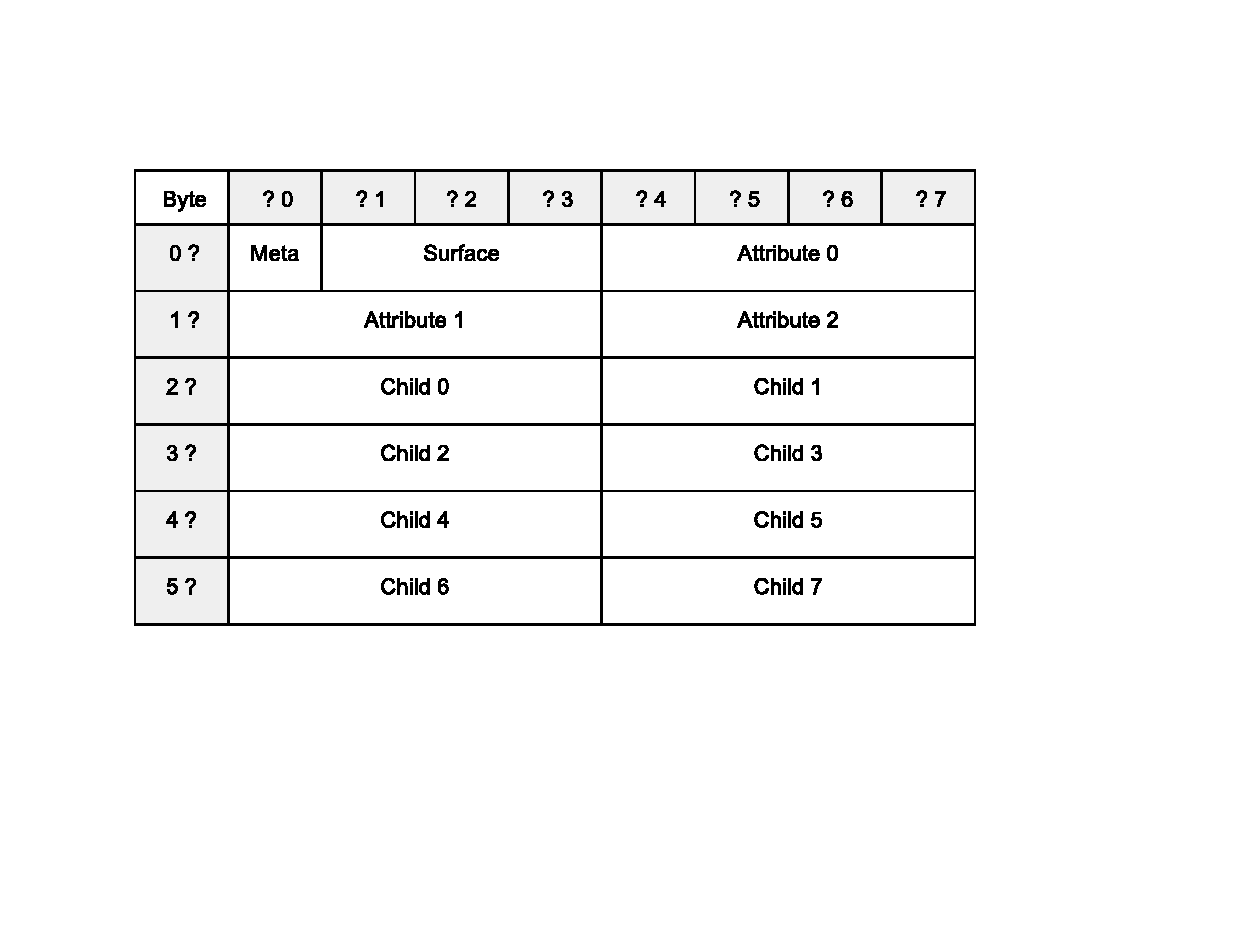
\includegraphics[width=\textwidth, viewport=50 120 475 380, clip=true]{nodeLayout.eps}
\caption{The data layout of a node. Byte positions are in octal for ease of representation.}
\end{center}
\end{figure}

The purpose of each of these fields is as follows:

\begin{itemize}

\item The meta value indicates the type of the voxel represented by a given node. This informs how data within each of the three attribute values are interpreted.
\item The surface value represents the normal of the surface represented by the voxel as well as the position of this surface within the voxel.
\item The attribute values, as stated previously, may be interpreted in a variety of ways depending upon the value of the meta value.
\item The child values are the offset of each child of the node in the data buffer, in units equal to the size of a node. Should the value of a child node be set to the maximum representable value for a 32-bit unsigned integer, this indicates that a child corresponding to this field does not exist. Considering such a node would theoretically be at the end of a buffer over 190 GB in size, which is well beyond the memory capacity of all current consumer graphics hardware, it is assumed such a node would not be created.
\end{itemize}


\foursection{The Head Buffer}

The Head Buffer is an array which stores the head node of each sparse voxel octree resident to the Voxel State.
This buffer exists to provide a means of simply indexing into the head nodes of each SVO, which is a necessary initial operation for manipulating or tracing through an SVO.\\


\foursection{The Heap Buffer}

The Heap Buffer is where references to free nodes in the Data Buffer are stored for retrieval by Yggdrasil as need for more memory arises.
The Heap Buffer houses an array of integers, grouped into sets of four, with a number of sets equivalent to the number of processor units present on the GPU.
When a process from Yggdrasil intending to manipulate the Voxel State runs on the GPU, it must necessarily be the only manipulating process running on the GPU at the time.
This is because each work item run during these jobs uses its global identification number to determine which of these sets of integers to use in order to get free memory.
See figure 2 for diagram.

\begin{figure}[H]
\begin{center}
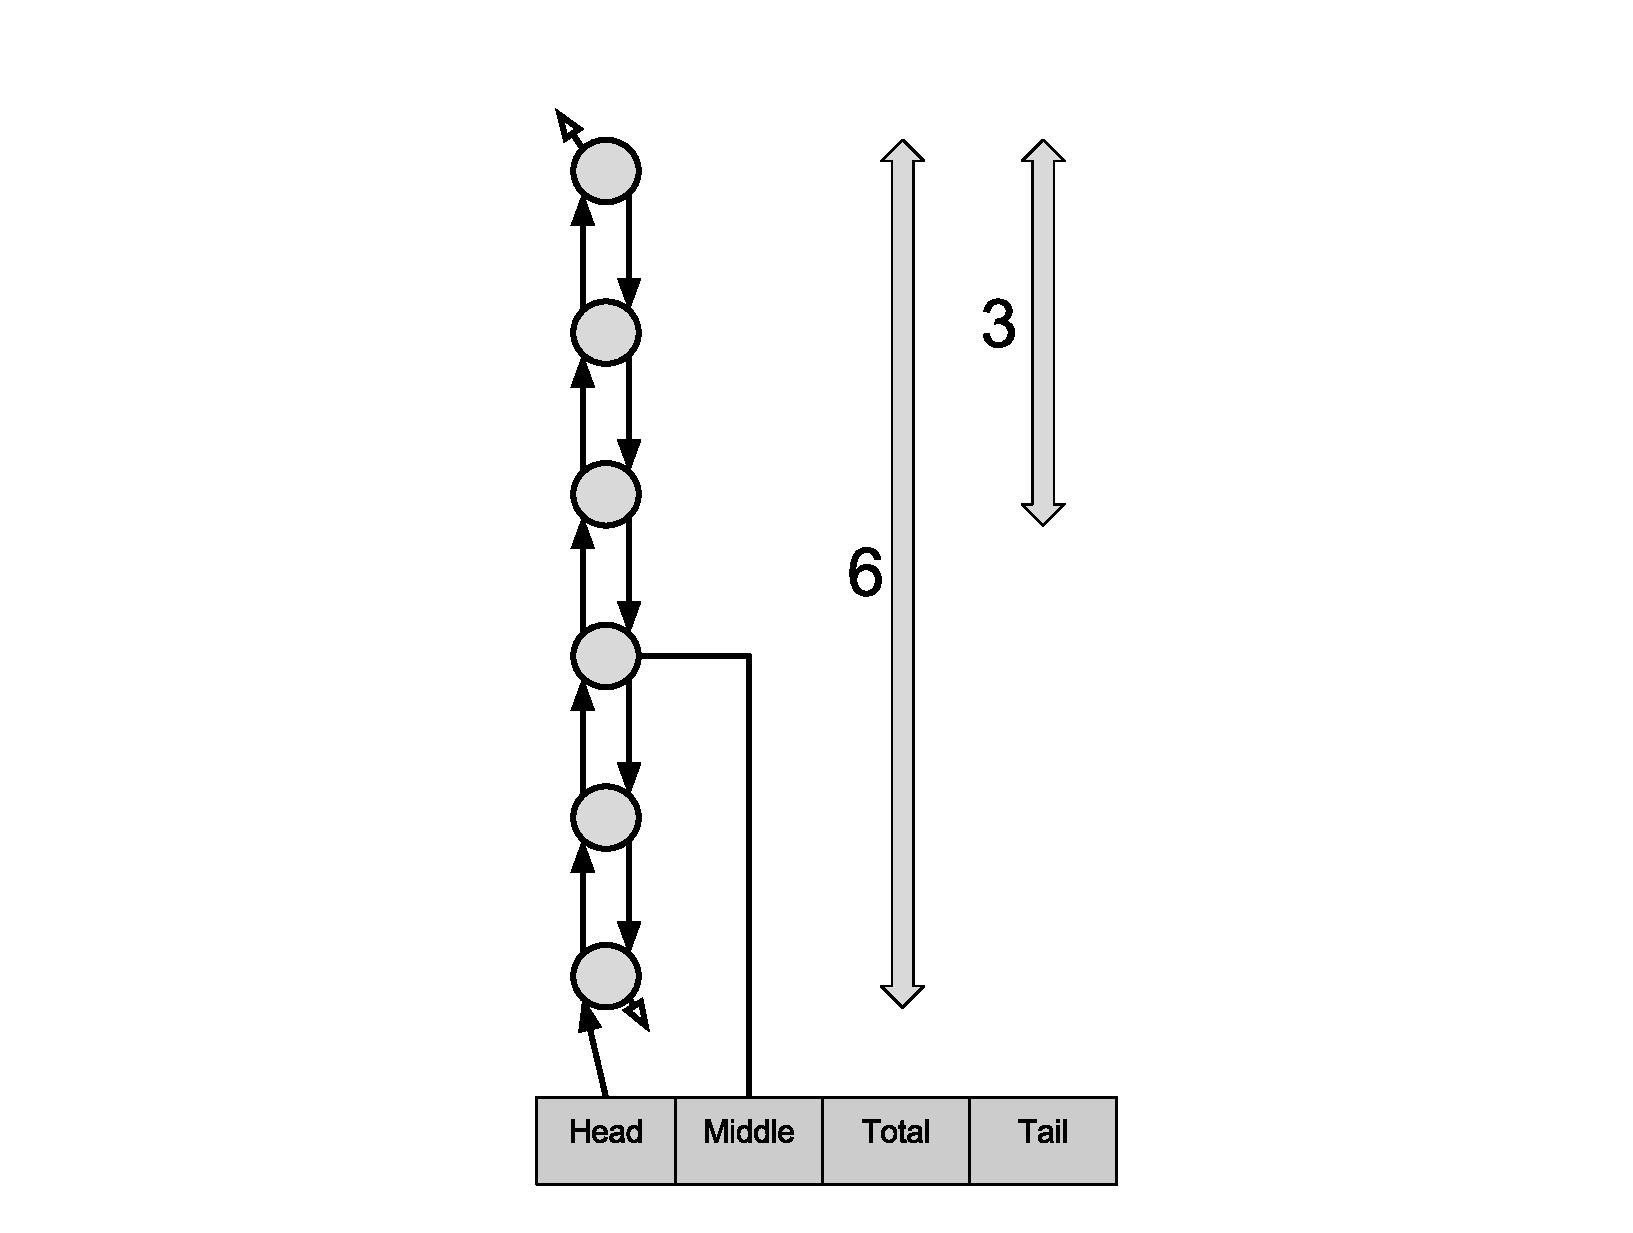
\includegraphics[width=\textwidth]{HeapBufferElement.eps}
\caption{The structure and nature of an element of the Heap Buffer}
\end{center}
\end{figure}

The first integer of these groups is the index of a node not used in the Data Buffer.
This node forms the head of a linked list of other nodes, with each node using the child 0 and child 1 fields of each node to link it to its headward and tailward neighbors.
Should the work unit corresponding to this triplet be in need of a free node, it retrieves the node from this index.

The second integer of these groups is the index of a node roughly in the center of the linked list indexed by the first integer.
This is done for list balancing, which is discussed in the Yggdrasil section.

The third integer indicates the number of links in the list pointed to by the first integer, whereas the fourth integer indicates the number of links following the link indexed by the second integer.
These are also used for list balancing.

When properly managed by Yggdrasil, the Heap Buffer provides constant-time access to each thread in the GPU and with no fragmentation among allocated memory, since allocating one node simply costs one nodes worth of memory.
This means that not only is adding and removing items from the octree quick regardless of how much memory is being used, but only the memory that is needed is allocated from the Data Buffer.

\threesection{Components of the graphics engine (Yggdrasil)}

Yggdrasil, named for the cosmic world tree of Norse mythology, is the framework of GPU-native programs that are in charge of managing and rendering the Voxel State for PolyVox.
As with the Voxel State, efficiency of memory usage as well as speed are strong design concerns.
For this reason, reducing function runtime per input as well as memory footprint required for operations is key.

\foursection{The Data Buffer}
The Data Buffer holds all of the nodes that PolyVox uses to represent the voxels being viewed and interacted with by the user.
Yggdrasil uses the position of a node in the Data Buffer when referencing it during Yggdrasil’s regular operation.
\foursection{The Head Buffer}
The Head Buffer is an array holding the index of the root of all SVOs present in the Data Buffer.
This is used to uniquely identify every SVO in the Voxel State and is used at the beginning of each operation to begin tree traversals.
\foursection{The Heap Buffer}
The Heap Buffer is an array holding references to the heads of a series of linked lists composed of nodes.
Additionally, next to each list reference is a reference to a link somewhere in the middle of the list, the number of links in the list, and the number of links between the second reference and the tail.
This additional data is used to keep the length of the lists in the Heap Buffer close to one another, ensuring heavily used lists do not quickly run out of links.
\foursection{The Tool Executer}
The Tool Executer is a general-purpose OpenCL program template for the application of arbitrary operations to the Voxel State according to the user’s brush strokes and the currently selected tool.
Whenever a new tool is loaded into PolyVox by the Interchange, the OpenCL code specific to that tool is injected into the template, which is then compiled into a tool executer.
Regardless of what code is injected, much of the operation of the tool executer is the same.

The Tool Executer is passed a number of inputs based off the state of the brush stroke being performed by the user.
This state includes what part of the stroke (beginning, middle, end) the operation is in, the line segment representing the path the stroke just made, the selected height, width, and depth of the brush tip used, the weight of the stroke, and the speed of the stroke.

Based on of the dimensions of the brush tip as well as the line segment representing the section of brush stroke just made, the Tool Executer traverses the SVO being actively edited, finding the smallest voxel in the octree which completely contains the bounds of the stroke section.
Once this voxel is found, the voxel is given to the first section of injected tool code, which determines how much further the Tool Executer traverses into the octee.
The code may either report that no more traversal is needed, or request further traversal.
This request will be refused if the maximum resolution depth has been reached.
If not, the Tool Executer allocates and attaches any missing child nodes, if necessary, then traverses into the nodes. This process is repeated until all traversals have reached bottom.

Once all Tool Executer traversals have reached their final depth, the voxels at the end of each trace are handed to a different set of injected code, which evaluates what the new state of each voxel should be.
Once the new states are assigned and the injected code passes back execution, the Tool Executer reverses its traversals, applying a third piece of injected code to each parent voxel, ensuring that each one has a high-level representation of its children.

Once all traversals have been reversed, the Tool Executer terminates.
\foursection{The Renderer}

The Renderer is the OpenGL program executed in order to create the imagery that appears to the user in their HMD.
The Renderer receives a set of triangles from the Interchange corresponding to the bounds of the SVO volumes visible to the user.
This means that SVOs which do not intersect with the near plane of the user’s vision would be represented as boxes.
Those SVOs that do intersect with the user’s near plane of vision would be represented as boxes truncated along the user’s near plane of vision.

Each of the vertices are given their corresponding position in the SVO as well as the index in the Head Buffer where the head of the box’s corresponding SVO is stored.
Using this data, the fragment shader traverses the SVO as a voxel cone trace.
As this trace is performed, for any given voxel it traces through, it will trace through its child nodes instead if that voxel has a cross section in the view projection larger than the fragment.
This trace is performed until the contribution of samples to the final value of the trace drops below the smallest nonzero value representable by the trace's alpha component.
Once the final value for a trace has been rendered, it is used as the color value for the fragment corresponding to that trace.\\

\foursection{The Memory Manager}

The Memory Manager is an OpenCL program which serves two purposes.
Firstly, it performs balancing operations upon the Heap Buffer, alleviating imbalances in how much memory is available to each work group.
Secondly, it provides information regarding the availability of memory in PolyVox to the Interchange, allowing the Interchange to take necessary action, such as calling for more memory, culling excess detail, or providing a warning to the user.
See figure 3 for diagram.



\begin{figure}[H]
\begin{center}
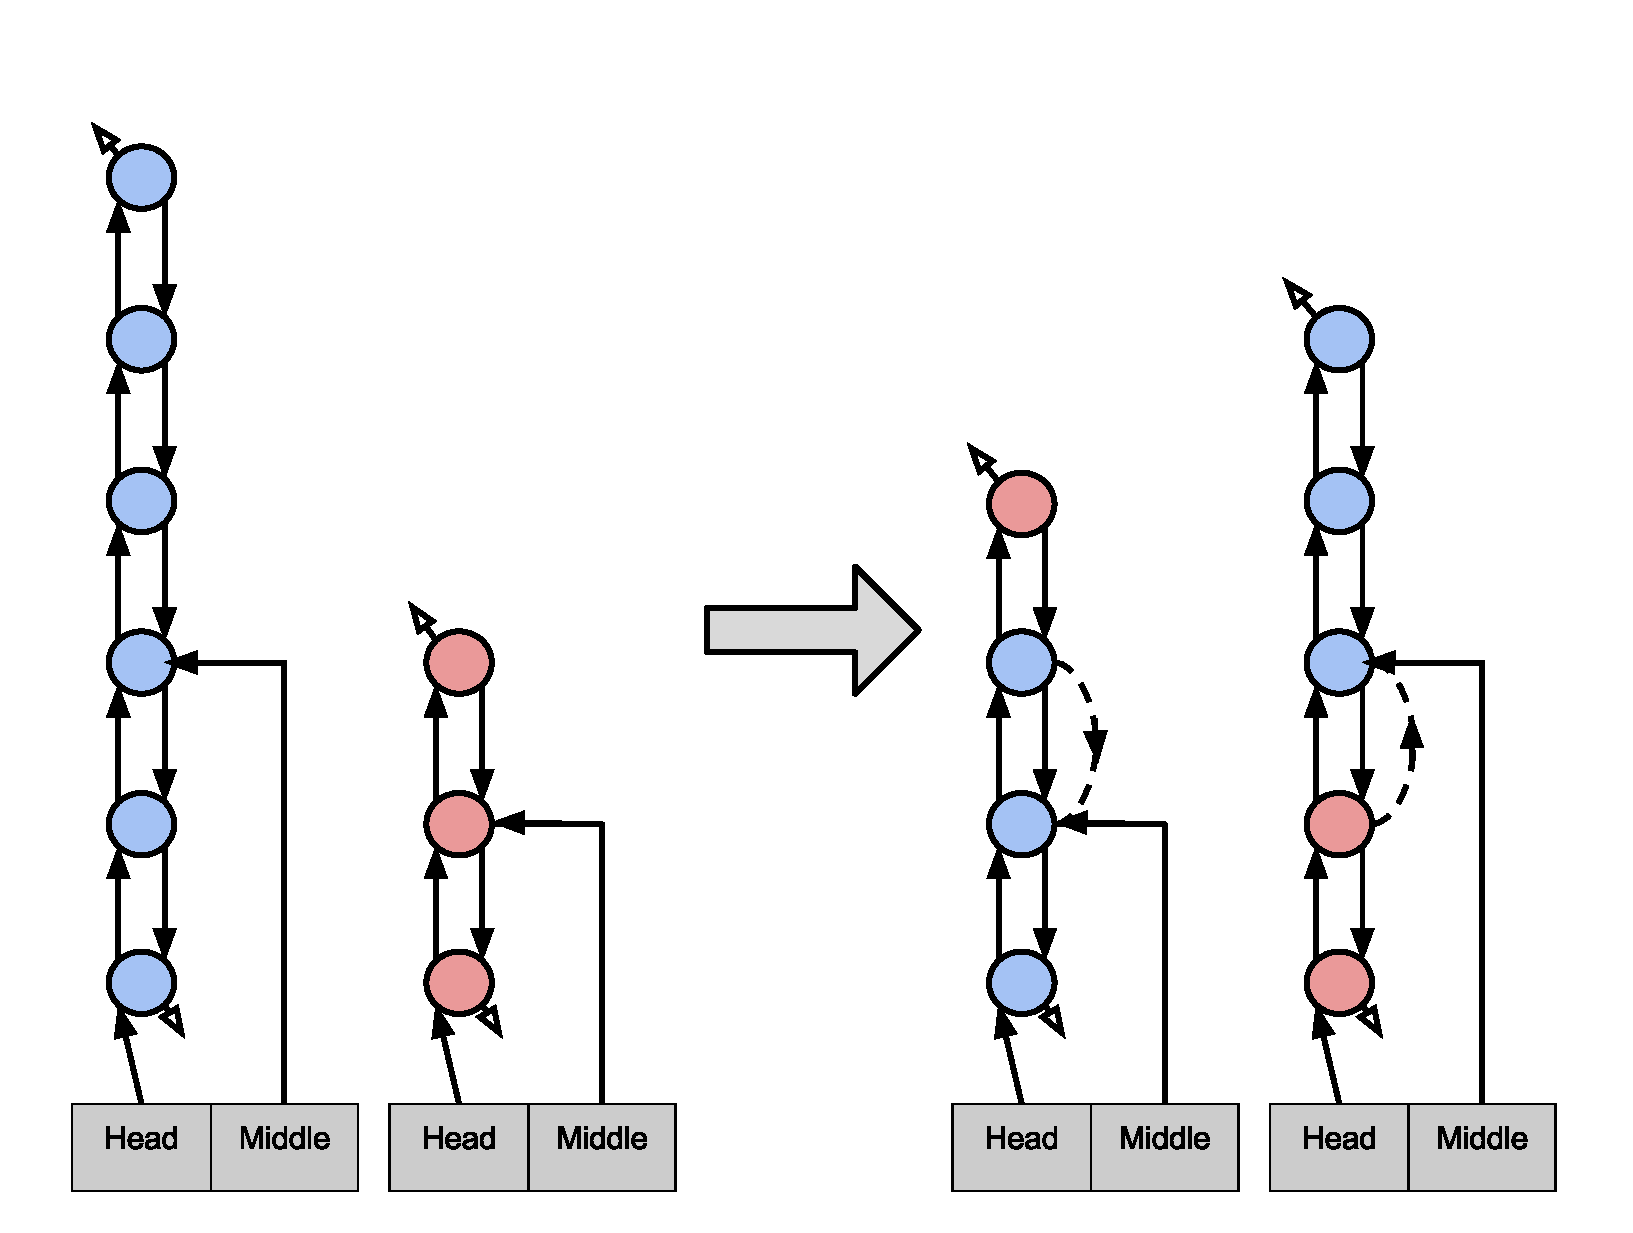
\includegraphics[width=\textwidth]{TailSwap.eps}
\caption{An example of a tail swap that could be carried out during a balancing procedure}
\end{center}
\end{figure}


The balancing procedure performed is relatively simple, each work item is given one of the linked lists.
These work items then establish their position in a binary tree, where work items with a global id, n, have work items n*2 and n*2+1 as children.
Work items at even depths in the tree inspect the data in its left child, retrieving the data member referencing a link in the middle of its linked list.
Using this reference as well as the reference to a link in the middle of its own linked list, the acting working group switches the links across the two lists, causing all trailing links to also be appended to the other list.
The link count members as well as the reference to the middle link for each work item are updated accordingly.

As stated previously, the middle links referenced for each linked list must be generally towards the center of the linked list.
This is why the reference is traversed up or down the linked list up to sixteen links in order to begin approaching the halfway point for each list.
This process is applied by the acting work groups to their right children, and these two processes are repeated by working groups at odd depths.
Repeating this process multiple times, exchanging the tail half of each list, rebalancing halfway link references, then exchanging again, causes links to be more evenly distributed across the Heap Buffer.

Once these exchanges occur the number of times requested by the Interchange, the minimum and maximum linked list size is calculated through reduction and returned to the Interchange.
This gives the Interchange a measure of how balanced the linked lists became as a result of the operation.

\threesection{Interactions between the hardware and the Interchange}
The VR HMD and motion controls act as the source of input for the user.
The VR hardware will primarily interact with the system using pre-built drivers for the Unity engine, which are both easily available and open source.
With such widely available device drivers, hardware implementation is, for the most part, a solved problem.
The primary challenge from a design standpoint is how signals sent from, and received by the program are handled.

\foursection{Design Entities}
\textbf{Vive HMD} \\
The HTC Vive needs to have the HDMI, USB cable, and power adapter attached to the Vive's link box. The link box is then attached to the computer with an HDMI cable and USB cable. This completes the connection between the HMD and the computer.\\
\textbf{Vive Lighthouses} \\
The lighthouses and the integrated VR tracking solution need to be mounted on the wall or with stands. They must be connected to power and programmed to ‘A’ and ‘B’ channels within the VR driver. They must also have a BNC sync cable running between them. If the sync cable does not fit the volume model, then we must use channels ‘B’ and ‘C.’ The light houses must be spaced at least 15 feet apart. 
\foursection{Design} 
The driver is operated by the Steam VR asset in the Unity add-on window. The driver takes in input through the HMD and uses the data to manipulate the camera rig object in Unity. The Steam VR library allows for controller input to be passed to the game engine. This input must then be mapped to a trackable object in Unity. This object can then be used by the Interchange for processing. The same process is performed using data sent by the HMD. The packets sent by the controllers and HMD will be done through USB and sent to the Interchange. We will need position and orientation of the HMD and at least on of the Vive controllers. We will also need trackpad and trigger inputs from the controller. This will be sent to PolyVox and into the Interchange driver.

\threesection{Architecture of the User Interface}
The UI will essentially be a game object that can be moved and accessed around the peripheral of the user. The user should have the option to specify rotation lock, where the UI object follows them everywhere they look. This allows the user to have access to the toolset at all times. Turning this off will only invoke position lock, where the UI object is always at a relative position to the user. 

\foursection{Design Entities}
\textbf{Brush Object} \\
Brush objects will be game objects operated by the UI and the game engine. Each brush object contains position and orientation of a motion controller, as well as whatever graphical transformations will be applied when a modify geometry command is sent via a button press.

\foursection{Design}
The UI will have two initial states, active and inactive. The inactive UI will be a small game object only capable of a few actions. The user can turn on or off the rotation lock. The user can move the UI object to another relative position while in this state. The state also has a way of moving the UI into the active state. 
The active state will have all of the same features as the inactive state, except that it can invoke the inactive state instead of the active state. It also can navigate a tree structure that gives the user access to all of the tools and environment settings. 

The UI response to track pad inputs on the Vive controller as well as the track pad target position. The trackpad press event. This acts as a confirmation operation when toggling states or selecting items in the UI. The UI will be structured to take advantage of non physical position dependence by allowing the trackpad to operate independently of the controller's physical position and orientation. This allows the user to operate the UI in the world space without relying on VR tracking.

The active UI design needs to be full capable of accessing all of the features in its layout. The layout will always have a button at the top for moving backwards. When at the top layer, this button moves from active to inactive. Each item in the UI will either be a UI element or a traversal node. The traversal nodes allow separation of UI pages and access to other nodes. The UI elements are access to settings and tools. UI elements can be things like brush type or brush color. See figure 4 for diagram.

\begin{figure}[H]
\begin{center}
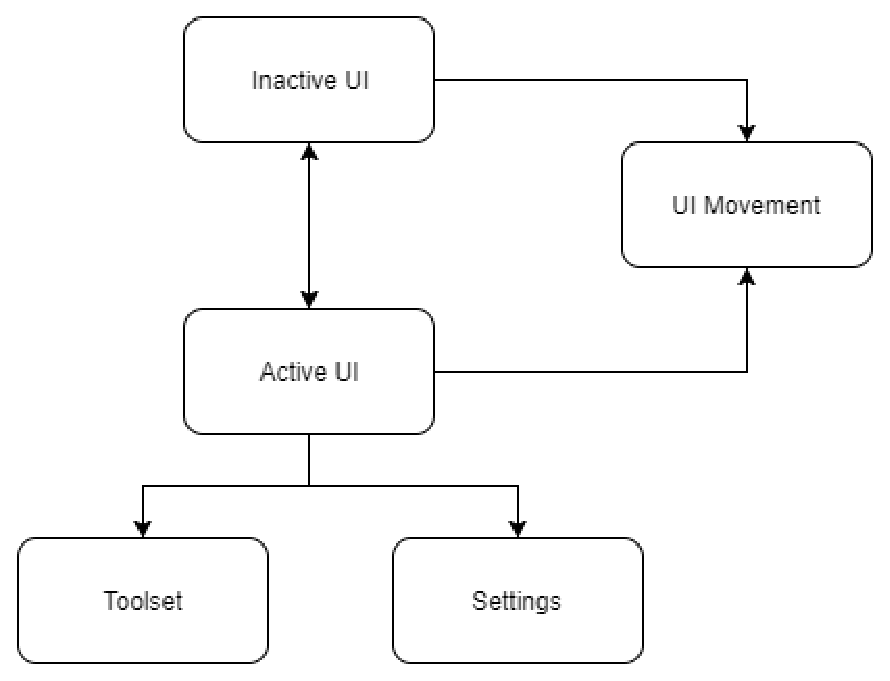
\includegraphics[width=\textwidth]{UIDiagram.eps}
\caption{An example of a tail swap that could be carried out during a balancing procedure}
\end{center}
\end{figure}

\threesection{Architecture of the Interchange}
The Interchange will be the primary point of communication and manager for the disparate elements of the program.
The Interchange must be able to receive information supplied via the user interface and interface hardware and relay the corresponding instruction to the Yggdrasil engine to properly render the scene, and is directly responsible for directing state transition of all other components
 Due to the experimental nature of the project, the design of the Interchange must be kept at a high level. Specifics of functions and the processing of data will need to be determined in development. 

The Interchange must be capable of properly coordinating all other elements of PolyVox as a whole, and is a central element  in executing commands supplied via user interactions, implementing program features, and directing the graphics engine’s rendering operations. As such it is relevant to design concerns of all stakeholders involved in the project. In particular, it is central to the operation of the user interface and motion controls, from which it will receive user commands, and the operation of the graphics engine, which it will send commands to. As the Interchange will be the point at which the program’s toolset is constructed, it will also dictate the program’s available features.

\foursection{Design Entities}
\textbf{Unity Engine:}\\
The Interchange will be built in and run on the Unity Game Engine.
Unity has its own proprietary rendering and modeling systems, as well as native compatibility with motion tracking systems and dual rendering used in VR.
Additionally, Unity has native scripting compatibility and will serve as the platform for developing the program tools and features.\cite{unity}\\
\textbf{C\#:}\\
C\# is one of the most frequently used languages for scripting in game engines, and is natively compatible with Unity.
Most features and tools for the program will be constructed using C\#. 

\foursection{Design}
When in operation, the Interchange will receive positional information from the user via both the HMD and VR motion controls in the form of four-element vector positional coordinates.
Using Unity’s native VR drivers, the Interchange will translate these coordinates into a position relative to the voxel state.

Additionally, the data received from the user may or may not include a user-inputted command via a button press.
When pressed, the button input will be sent to a function, which is also passed the current state of the UI (such as what ‘brush’ is selected, or what menu the user currently has open).
The function will process the user command to determine any possible UI state changes, as well as any changes to the voxel state the user command will perform (such as creating or destroying a voxel) based on whatever tool or UI element is currently being operated. 

Any changes in the state are returned by the function as a set of commands to the graphics engine.
The graphics engine will then process the commands from the Interchange.
Before the render is sent to the HMD, the graphics engine will return a flag that will determine if the Interchange needs to perform additional actions, such as sending a command to the GPU to allocate additional memory.
If so, the Interchange will send the appropriate commands, and the graphics engine will reattempt the render. This repeats until the flag sent from the GPU is null. 

While the operations of the Interchange are primarily just in service to other elements of the program, they are still vitally necessary to PolyVox’s operation.
The Interchange effectively acts as the driver for the graphics engine and the motion control system, and is needed in order to develop a working feature set and comfortable user interface. 
See figure 5 for diagram.

\begin{figure}[H]
\begin{center}
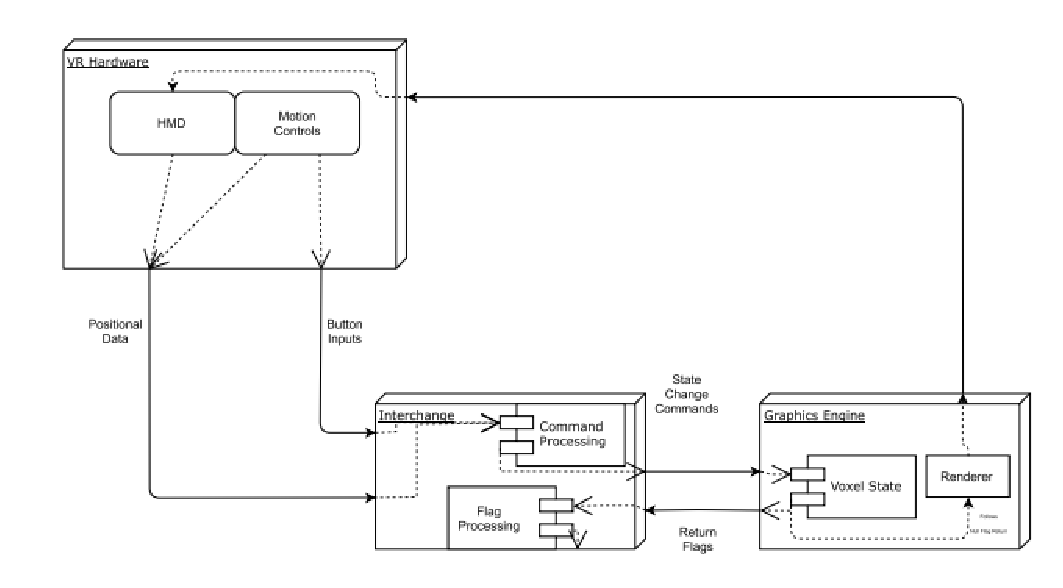
\includegraphics[width=\textwidth]{Interchange.eps}
\caption{General architecture of the Interchange}
\end{center}
\end{figure}


\subsection{Current Design}

\subsubsection{Introduction}

\threesection{Purpose}
This Software Design Description (SDD) specifies the design plan for the VR based 3D art program PolyVox as of June 12, 2018.
This document expands upon the content of the PolyVox Software Requirements Specifications (SRS), and specifies how the elements of the SRS are incorporated into the program.

\threesection{Scope}
This document describes the structure of PolyVox and the implementation of its individual components.
This document assumes that any reader is already familiar with the PolyVox SRS and the project as a whole.
This document, in its creation, was intended to be included as part of a larger collection of works comprising a final report, including the original design document.
Due to this, pieces of information that have already been included in the original design document which have not changed, such as the glossary of terms and project stake holders, have been omitted to reduce redundancy under the assumption this information has already been encountered.

\threesection{Intended Audience}
This document details the technical design of the PolyVox application, and, as such, is intended for readers with knowledge of programming and software development methods. 

\subsubsection{The Front End}

The application layer will be the primary point of communication and manager for the disparate elements of the program.
This level of the system must be able to receive information supplied via the user interface and interface hardware and relay the corresponding instruction to the ray tracer to properly render the scene, and is directly responsible for directing state transition of all other components. 

The application layer must be capable of properly coordinating all other elements of PolyVox as a whole, and is a central element in executing commands supplied via user interactions, implementing program features, and directing the graphics engines rendering operations.
As such it is relevant to design concerns of all stakeholders involved in the project.
In particular, it is central to the operation of the user interface and motion controls, from which it will receive user commands, and the operation of the graphics engine, which it will send commands to.
As the Interchange will be the point at which the programs toolset is constructed, it will also dictate the programs available features.

\threesection{Design Entities}
\foursection{Unity Engine}
 The Interchange will be built in and run on the Unity Game Engine.
Unity has its own proprietary rendering and modeling systems, as well as native compatibility with motion tracking systems and dual rendering used in VR.
Additionally, Unity has native scripting compatibility and will serve as the platform for developing the program tools and features.
\foursection{C\#}
 C\# is one of the most frequently used languages for scripting in game engines, and is natively compatible with Unity.
 Most features and tools for the program will be constructed using C\#. 

\threesection{Design}
When in operation, the application layer will receive positional information from the user via both the HMD and VR motion controls in the form of four-element vector positional coordinates.
Using the SteamVR and OpenVR libraries, the application layer will translate these coordinates into a position relative to the voxel state.
Additionally, the data received from the user may or may not include a user-input command via a button press. Unity handles VR controller input via scripting events.
Our system implements event listeners which trigger handlers when input is detected.
These event handlers will trigger functions, which alter the state of the program.
This state would include factors such as the scale and color of the brush, or what menu the user currently has open.
These functions will process the user command to determine any possible UI state changes, as well as any changes to the voxel state the user command will perform.
Any changes in the state are returned by the function as a set of commands to the graphics engine.
The graphics engine will then process the commands from the application layer.
While the operations of the application layer are primarily just in service to other elements of the program, they are still vitally necessary to PolyVox’s operation.
The application effectively acts as the driver for the ray tracer and the motion control systems, and is needed in order to develop a working feature set and comfortable user interface.


\subsubsection{Interactions between the Hardware and Application Layer}

The VR HMD and motion controls act as the source of input for the user.
The VR hardware will primarily interact with the system using pre-built drivers for the Unity engine, which are both easily available and open source.
With such widely available device drivers, hardware implementation is, for the most part, a solved problem.
The primary challenge from a design standpoint is how signals sent from, and received by the program are handled. 

\threesection{Design Entities}

\foursection{Rift HMD} 
The Oculus Rift needs to have its HDMI and USB 3.0 cables attached to the computer.
This completes the connection between the HMD and the computer. 

\foursection{Oculus Sensors}
The sensors and the integrated VR tracking solution need to be mounted on the wall or with stands. 
The first two connected must utilize USB 3.0 ports, while the third will use a USB 2.0 port.
The first two sensors should be placed approximately seven feet apart, both facing toward the center of the ‘play space’.
The third should be placed such that it is approximately seven feet from the rightmost sensor (when facing the first two sensors) and approximately ten feet from the leftmost sensor.

\threesection{Design}
The driver is operated by the SteamVR asset in the Unity add-on window.
The driver takes in input through the HMD and uses the data to manipulate the camera rig object in Unity.
The SteamVR library allows for controller input to be passed to the game engine.
This input must then be mapped to a trackable object in Unity.
This object can then be used by the application layer for processing.
The same process is performed using data sent by the HMD.
The packets sent by the controllers and HMD will be done through USB and sent to the Interchange.
We will need position and orientation of the HMD and at least on of the Vive controllers.
We will also need trackpad and trigger inputs from the controller.
This will be sent to PolyVox and into the application layer.


\subsubsection{The Back End}

\threesection{Design Entities (Data Representation)}

To meet the performance demands of PolyVox while still creating a worthwhile experience, including high resolution and flexibility, a framework was constructed that can efficiently process the actions required of PolyVox.
This framework, given that it represents the lowest position in the hierarchy of abstraction the project deals with, was dubbed the back end.
It was concluded that the back end should accomplish its duties through parallel processing in GPGPU programs because it includes both the manipulation and rendering of potentially vast amounts of data, which can stand to benefit from the parallelism offered by GPU processing.
This decision means that the data associated with the world data of PolyVox is largely contained within the GPU itself and hence requires parallel-friendly means of access and manipulation.
The operation of the back end is broadly encapsulated in three main roles: data representation, data manipulation, and rendering, as described below.

\foursection{Voxels}

The back end represents the state of the 3D space being manipulated with voxels, cubes of uniform size forming a regular grid, with each cube having a certain state associated with it that characterizes the cube’s contents.
Voxels were chosen due to their ability to represent data volumetrically rather than by describing surfaces.
Numerous other methods could be applied to represent painted material in a 3D space;
however, using voxel representation means that volumetrically oriented operations, such as depositing or removing material in the space, which is likely to be frequently applied during the use of PolyVox, will be easier to perform.

The material properties of a voxel are represented by color and surface.
The color of the material represented by a voxel is encoded as a series of four floating point values, each respectively encoding a red, green, blue, and alpha channel.
The first three of these channels indicate the color of a voxel, as expressed by three additive primary colors of human vision, whereas the last channel represents how opaque the voxel is to light transmission.

The way an object’s contours are shaded depends upon the direction in which these contours face, otherwise known as their normals.
The surface property of a voxel is an encoding of a normal and is a vital piece of information for calculating shading of the boundaries between different colors of voxels.
This is because, the more a surface faces towards a light source, the more that surface is lit by that light source, assuming the incoming light is unobstructed.
This surface normal is represented as series of three floating-point values, an X, a Y, and a Z, that are used to form  a normalized vector.


\foursection{3D Textures}
For the sake of simplicity and rapid data access, the data associated with voxels are stored in a 3D texture, thus allowing programs in the back end to reference the data of specific voxels by indexing into the texture the three dimensional coordinates of that voxel.
The overall size of data associated with a 3D texture is limited. Thus, for the sake of increasing the number of voxels that may be referenced at a given time, the color and surface properties of voxels are broken into two separate 3D textures.
In addition to these components, an additional 3D texture is used to encode metadata about the contents of the other two textures.
More regarding this texture is discussed later in the data manipulation and rendering sections.

\foursection{Blocks}
The environment represented by PolyVox may not be small enough to fit on a single set of 3D textures because 3D textures can be limited in how much data they may contain effectively, the entirety of;
therefore, the three types of 3D textures associated with a section of voxels are bundled together and encapsulated in an object class called a block.
Thus, the geometry data of PolyVox is organized as a grid of grids, with the contents of individual blocks being operated upon independently during rendering and manipulation while the voxels encoded in a block encode the specific elementary units which the user may interact with. 
Blocks collectively represent a continuous grid of voxels in the space, each containing a set of 3D textures, all of equal dimensions and, themselves, scaled and arranged in space as a grid of cubes.

\threesection{Design: Data Manipulation}

\foursection{Wiping}
The first and also simplest form of data manipulation applied to blocks is what is referred to as a wipe operation.
A wipe operation simply writes a preset color and surface value to all voxels in the block.
Wiping is useful for clearing a texture either during the start of its use or just prior to loading in a saved state.

\foursection{Brushing}
The brush operation is what updates a block to reflect the stroke performed when the user paints in the space of PolyVox.
A brush stroke is described by four main pieces of information: a starting transformation, an ending transformation, a starting color, and an ending color.
The starting and ending transformations are each four-by-four matrices describing the transformation of the brush tip in the space of PolyVox, with the starting transformation indicating the transformation of the brush in the prior processing pass and the ending transformation indicating the transformation of the brush at the current processing pass.
Likewise, the starting and ending colors are each a set of four floating point values encoding an RGBA quadruplet indicating the color and transparency of the material deposited by the brush at each endpoint in the stroke.

Given the input transformations, the brush shader finds the point in time when each voxel is closest to the center of the brush, assuming that the start point of the brush is at a time 0 and the ending point of the brush is at a time of 1.
Given this information, an interpolation between the starting and ending transformation is found using the time metric as an alpha value, thus rendering the the transformation along the stroke during which the voxel was closest to the center of the brush.
Applying the inverse of this transformation on the position of the center of the voxel in question, one finds what is referred to as the voxel’s brush space coordinates.
From there, the voxel is considered to be affected by the brush if it exists inside the unit circle of its brush space.

The normal of the voxel, if it is determined to be affected by the stroke being processed, is then calculated by taking the normalized displacement of the voxel from the center of the brush.
This brush-space normal is then converted to world-space coordinates through a normal matrix, which is found by applying the transpose of the interpolated brush transformation.
This world space normal is what is ultimately stored because it makes consistent normal-based lighting simpler to carry out.

Once the normal of a voxel has been found, it is stored in the voxel’s corresponding element in the surface texture of the voxel’s respective block.
Likewise, the color of the voxel is found by interpolating between the starting and ending color by the time metric previously mentioned.
Thus, the material properties of all voxels now account for the new brush stroke defined by this operation’s parameters.


\foursection{Updating the Skip Grid}
As mentioned previously, there is an additional 3D texture associated with each block, in addition to the two that respectively represent the color and surface properties of voxels.
This texture, referred to as the Skip Grid, stores metadata describing patterns of similarity within the properties of regions of voxels.
This set of data is included because it allows the program in charge of rendering for PolyVox to perform ray tracing operations to approach log(N) running time in most use cases, with N being the number of voxels between a trace’s start and eventual end.
Generally speaking, the specific role of such a data structure as well as what information it represents would be mentioned in the data representation section, but the definition of the data has a degree of nuance and is best represented by describing the program in charge of calculating this data.
Thus, the definition of the Skip Grid has been fully relegated to this section.

In broad terms, a Skip Grid represents two concepts: whether or not regions of voxels are similar and whether or not regions of voxels are fully surrounded by a layer of voxels similar to its contents.
Simply put, these properties are described as local similarity and coverage, respectively.
To keep the runtime of calculating these properties small and the data layout easy to represent, the Skip Grid represents only the local similarity and coverage of cubic regions of voxels with power-of-two side lengths that have a minor corner offset from the origin by some integer multiple of this side length.
By setting this restriction, the processing of this information can be performed through reduction, whereby every cube of side length two is tested for local similarity and coverage and every cube with a higher side length may have their local similarity and coverage calculated by checking if all smaller cubes contained within the bounds also have local similarity or coverage and possess the same color.

Whether the surface properties of voxels are checked for similarity when evaluating local similarity is dependent upon the whether the cube currently being processed is covered.
This caveat presents a challenge:
If this cube is covered, surface properties are not checked because coverage effectively means that the cube under consideration is inside a region of similar material, and hence does not represent a surface to begin with.
Otherwise, the surface properties of the cubes are checked for similarity.
This addition to the process of generating a Skip Grid is useful because it finds larger regions of effective local similarity and hence can speed up ray tracing even more.


\threesection{Design: Rendering}
\foursection{Fragment Generation}
The ray tracer is exposed to the user by incorporating the ray tracer into a specific material that is rasterized onto the scene.
This method of fragment generation is applied because the voxels present in a PolyVox scene are not the only things visible to the user and that the other elements comprising the scene are rendered via raster graphics rather than ray tracing.
This material is given to the models of block objects, which are simple cube models, and the initial position and direction of the ray trace relative to the contents of the block’s 3D textures is determined by the generated fragment’s color and worldspace coordinates, respectively.

\foursection{Ray Trace Traversal}
When designing the ray tracer, a central heuristic was to minimize required processing without degrading accuracy.
Thus if a large set of redundant steps can be reduced to much fewer, slightly more complicated steps, the ray tracer should account for it.
The result is a ray that traverses the set of voxels within a block is from boundary to boundary, where each step in the trace is as long as it can be without exceeding the bounds of a region of similarity.
Thus, if a trace is traversing through a region of space with large pockets of completely transparent voxels,  the trace should travel faster through these pockets as the Skip Grid would inform the trace that it may extend the length of its steps to match the bounds of the similar regions.

Generally speaking, most use cases for PolyVox likely involve large swaths of space with the same color mainly because many of the scenes or objects that most would wish to prevent would be surrounded by or filled with empty space or air, just as most things in the universe are. For instance, one would find it strange if the inside of a building, the space above a street, or the region above a landscape were not mostly air. It is for this reason, as well as the need for higher processing speed, that the Skip Grid and this mode of traversal were incorporated into PolyVox.


\foursection{Processing Ray Trace Steps}
As stated above, each step made by the ray tracer is guaranteed to travel only through regions of similar material properties, which means that the state of the trace can be be altered as though the regions were simply one voxel.
Given this, a trace can be broken down into its individual steps and processed by calculating each step in order from the steps closest to the camera to those furthest away.
As each step is processed, the color of the region being traversed is fetched from its place in the 3D texture representing color and is then multiplied by an ongoing alpha value.

This alpha value starts at 1 at the start of the trace and decreases as time goes on, where the alpha is multiplied at each step by a factor of (1 - A)L where A is the alpha value of the material being traced through and L is the distance traversed in the step.
Distance is accounted for in this process because the amount light is not occluded by a material of some transparency follows a decay curve as the distance traversed becomes greater.

Additionally, if the ray tracer finds that a trace is traversing a region of space that is not considered covered, the color of the material, excluding the alpha, is divided by the dot product of the surface normal and the normalized displacement of this voxel from the light source. This essentially means that the ray tracer calculates a simple diffuse lighting effect for every voxel it encounters that is at a boundary of similarity, which can provide a greater sense of depth to the scene by giving objects shading.


\foursection{Render Ordering}
A final aspect of rendering voxels to consider is the ordering of rendering ray trace fragments to the screen.
This is actually handled by Unity itself, because the material which the ray tracing shader is associated with is given flags to indicate that it has transparency and so indicates to Unity that it should apply the painter’s algorithm to the blocks, painting them from back to front.

\pagebreak
\section{Technology Review}

\subsection{Christopher Bakkom}
\subsubsection{User Interface}
This project will be using a game engine to help produce the final product. The game engines we have chosen, based on popularity, documentation, and VR integration, are Unity, Unreal and the CryEngine. Each of these has their own way of creating a user interface. Important things to keep in mind is how they can be interacted with. Since we are using virtual reality, it will be important that these UI's be flexible enough to use the input from a wide variety of sources. All three of the game engines referenced in this section are free to use for our type of project.

\threesection{Unity}
Unity uses a custom game object inheritance to define it's user interface models. The objects created can have custom visuals and interaction. Each button in the toolkit has an onClick even, that can give custom commands. There is also support for all kinds of screen manipulation and custom animations. This will be useful in provide support for tools that may not be as precise. Unity has full support for built in VR user interfaces. There are clear definitions for non-dietetic UI, that can overlay menus that do not exists in the world. This will be very useful when a heads-up display for editing functions.

This infrastructure provides some easy support for what we are trying to do. It would be the optimal choice for minimizing the time we spend on creating the user interface. With the open integration of VR interfaces, the Unity engine is my top choice for our UI. 

\threesection{Unreal}
While the Unreal Engine doesn't have direct support of a UI, it does have a supported toolkit layer called UMG that provides the necessary functions. This is similar to a UI toolkit like Qt or MFC. This layer integrates with Unreal Engine while having its own separate code for customizing widgets, animation and events. There are tools for non-dietetic UI and in world space UI, but current this is still experimental in version 4.8. Epic games is releasing their Dragonfly Project that will show how these features can be used, however, the best we can hope for at the moment is community driven development on integrating these features.

Because of the short comings in Unreal's user interface it is probably not the best choice. It requires knowledge about this abstraction layer of UI and more work to do because it is not directly integrated into the engine. However, it is still a viable option for a user interface and could be used if the Unreal engine provides a benefit above the other engines in another way.

\threesection{CryEngine}
The CryEngine takes a similar approach to Unity in having all of its accessible features as close to the game engine as possible. UI elements are located in the game sdk files and all C++ source code is readily available. CryEngine has already solved some of the problems with the previous game engines by defining a UIEntity as a game object. This can be placed either in world space or non world space. This allows for custom UI interfaces that can be intractable as well as event driven in the world itself or outside of it in a 2D menu system.

While the CryEngine does have some great flexibility in its user interface, the learning curve for the CryEngine is steeper than most models. If we do decide to use the CryEngine we will have support for any kind of interface we want. The would be the optimal choice if we are trying to define a UI that is very unique and difficult to implement in the other engines

\subsubsection{VR Head Mounted Displays}
This section looks at the different specifications for the head mounted display for our user. When using and HMD, it is important to note the available compatiblity with our game engine as well as accuracy of the tracking solution and performance. We are trying to create an editing environment so being able to display fully rendered environments will need to be carefully considered when judging game engine integration. The project defines a user tests to be conducted at the end so there needs to be a realistically high standard of accuracy for this type of display. Price, although not a prime goal of this project, will also be a consideration.

\threesection{HTC Vive}
The HTC Vive is one of the most popular and highly rated VR headsets on the market, priced with the tracking and controllers at six hundred dollars. It has 2160 x 1200 resolution at 90hz with 110 degree field of view. The tracking technology includes a gyroscope, accelerometer, front facing camera and lighthouse tracking solution. This tracking provides a space of 15 x 15 feet. The PC requirements include a NVIDIA GeForce GTX 970 or a Radeon 480 or better, Intel i5-4590 or better and 4GB of RAM. Vive has been working to integrate with Valve's Steam platform to create libraries for development. It has supporting plugins for all three of the game engines listed above.

Because of the Vive's already integrated tracking, this is the most optimal solution for fast development. The plugins are readily available for every game engine, it has a great resolution and high refresh rate. What really puts it ahead of the Oculus Rift is the larger volume, which would help for a more immerse editing environment. This allows the user a greater amount of freedom.   

\threesection{Oculus Rift}
The Oculus Rift is priced at five hundred dollars with it's controllers. It has a resolution fo 2160 x 1200 at 90hz and a 110 degree field of view. It's tracking solution includes an accelerometer, gyroscope, and the Constellation camera tracking system providing up to an 8 x 8 feet environment. It requires an NVIDIA GeForce GTX 960 or a Radeon RX 470 or better, an Intel i3-6100 or better and 8GB of RAM. Oculus has been working to create a VR standard with WebVR and has support for many titles for its platform. It also has software plugins for all of the game engines listed above.

Where the Oculus Rift does well is its lower machine requirements. A lot of the benefits are similar to the Vive, but it is slightly cheaper to produce a machine to run it. However, these are minor benefits and not the purpose of our project. It has a huge down fall in that it drastically cuts down the viewing environment. We would need to implement another tracking solutions to improve this, which undermines the Oculus benefits. We would only use this if we are really having trouble getting a high powered computer.

\threesection{Gear VR}
The gear VR is one of the cheapest solutions at 100 dollars, that is with out the galaxy note required to power it ranging from 200 to 500 dollars. It has a 96 degree field of view and the resolution depends on the phone running it, but the minim is 2560 x 1440 running at 60hz. The lower frequency and resolution might make computation thresholds easier to work with in our application. Since the gear VR has similar SDKs to the Oculus, all of the supported software so far is mostly compatible between the two. This might be important for creating a modular system for integrating furtherer editing tools. There is the down side of the limited tracking in which the system would have to piggy back off of another tracking solution.

Because of the limited VR tracking for the Gear VR, this is probably not the best solution. If we were to implement the Gear VR, we would have to implement another tracking solutions that makes up for the lack of tracking in the Gear VR. This is do to the lack of position data given back by the Gear system. If we wanted to track only by motion capture, then we could consider this because of its low price and accessibility. 

\subsubsection{Object Tracking}
This section will look into the different ways this project can capture physical objects and represent them digitally. Our user will be able, at the minimum, interact with a user interface and create brush strokes in a 3D environment. These interactions are definable as operations take in the physical environment and then transfered to the editor. This section focuses on the established controllers provided by Oculus and HTC, motion capture and the DodecaPen presented by Oculus research. 

\threesection{Integrated VR Tracking}
The most obvious solution would be the controllers that the Oculus Rift and HTC Vive already provide. These controllers are tracked by the lighthouse and constellation tracking solutions. They also have their own analog and digital buttons that relay input to their respective SKDs. This would be the simplest solution because it would require much less compatibility modifications for the game engines. Because the SDKs already have the plugins established with the game engines, the digital inputs can already be accessed fairly easily.

Because this tracking solution is already available to us if we choose the Vive or Oculus, this is the most optimal for fast development. The support for this kind of tracking is already integrated into the VR headset and game engines. This should be our choice, unless we decide that we want to track other kinds of objects in the volume. Even if we want to to support other tracking solutions for other objects, we can layer these kind of features on top of the integrated VR tracking solution.  

\threesection{Motion Capture}
Mocap or motion capture, is a tracking solution that requires cameras and a higher demand for volume preparation. It also requires a high computation standard and would likely need it's own system. It is also one of the most costly solution as a high end mocap system can cost more that 100,000 dollars. Despite the overhead, motion capture makes up for it by being on of the most accurate tracking solutions on the market. There are lots of options for tracking active and passive markers placed on the object and even HMDs, providing better head tracking that the integrated solutions. It also has the benefit of being enormously flexibly, allow us to capture and track any physical object we want. This could open up a variety of different features not limited to just the brush. 

This is one of the most optimal tracking solutions as far as accuracy and flexibility. However, it requires huge amount of set up, access to a volume and it is very costly. We should only use if we already have access to all of these requirements and have time to integrate this kind of system. 

\threesection{DodecaPen}
The DodecaPen is a 6 dof tracking solution, research by the Media IC and System Lab at the National Taiwan University and the Vision and Learning Lab at the University of California at Merced. It uses geometric hexagon solid with QR codes to identify each face on the end of a pen to get 6 degree of freedom tracking. There has been some very promising results, stating high accuracy with only using a web cam costing less than 100 dollars to capture the solid. This research is still very experimental and there isn't a marketable solution yet. So integrating this piece of technology, despite the calculations being completely open, would not be an easy feature. It would require image processing and custom code to interpret the data. This could probably be a project on its own, but it is one of the most promising tracking solutions for our type of application to date. 

This is great tracking solution because of its low cost and accuracy. The only downside to this is that we would have to figure out how to integrate it ourselves. The Dodecapen is still experimental and although the solutions is completely open, there is no available software for us to use. We would have to figure out how to capture frames, do image processing and then do the calculations for six degree of freedom for this object. This should only be used as a last resort if for whatever reason every other tracking solution fails or we have ample time to integrate such a complicated system.

\newpage
\subsubsection{References}
~\\ 
Interaction Components Unity Technologies - \\
https://docs.unity3d.com/Manual/UIInteractionComponents.html \\ \\

User Interfaces for VR\\
https://unity3d.com/learn/tutorials/topics/virtual-reality/user-interfaces-vr\\ \\


UMG UI Designer\\
https://docs.unrealengine.com/latest/INT/Engine/UMG/index.html \\ \\


Creating 3D Widgets \\
https://docs.unrealengine.com/latest/INT/Engine/UMG/HowTo/Create3DWidgets/index.html \\ \\

User Interface - Technical Documentation \\
http://docs.cryengine.com/display/SDKDOC4/User+Interface \\

Oculus Rift vs. HTC Vive: Prices are lower, but our favorite remains the same \\
Digital Staff - https://www.digitaltrends.com/virtual-reality/oculus-rift-vs-htc-vive/ \\ \\

DodecaPen: Accurate 6DoF Tracking of a Passive Stylus \\
https://research.fb.com/publications/dodecapen-accurate-6dof-tracking-of-a-passive-stylus/ \\

\pagebreak
\subsection{Richard Cunard}
%\bibliography{richardTechRev}{}

\subsubsection{Scripting Language}

\threesection{Overview}
The choice of what programming language to use for developing our project will heavily inform the design and functionality of our final product. The goal of the project from a development perspective, is to create an efficient, stable, and flexible program. Any game engine available to the team will have a set of natively compatible scripting languages, which further narrows the choices available to the team.

\threesection{Criteria}
The primary factors each should be judged on are speed of code execution, robustness of features, and ease of development. Depending on the language, the output of the code can have wildly differing execution times. Given the requirement of maintaining a high frame rate, this is a significant factor in deciding the language. The feature set of each language will significantly affect how the program is constructed, and can help or hinder various aspects of development. Finally, assuming the first two criteria are met, the decision should be based on the how challenging development is with a given language.

\threesection{Potential Choices}
With that in mind, the most viable options for use in the project ar C$++$, C\#, and JavaScript. Each of these are robust, heavily supported languages, with large selections of publicly available libraries. More importantly, each is used natively in at least one major game engine. Choosing which of the three languages will likely also inform what game engine is chosen for the project, given that certain languages are either poorly supported, or simply incompatible with specific engines.

\foursection{C\#}
C\#, similar to its predecessor C$++$, is a powerful object oriented language with extensive functionality and outside support. C\# is supported by most modern game engines, including Unreal, Unity and CryEngine, which would present the team with more flexibility for future development choices. As mentioned above, while C\# is interpreted, it has several optimization features. These include the ability to query machine specifications, perform runtime code optimizations that would not be possible with a compiled language, and perform heap more efficiently. While the team has very limited experience with C\#, this would not seriously affect development, as it is similar in syntax and design to C$++$, which the entire team has extensive experience working with. C\# would be a viable choice for any choice in game engine and design methodology.\cite{richTech1}\cite{richTech2}

\foursection{C$++$}
C$++$ is a powerful language with extensive outside library support, and a fundamental compatibility with the Unreal Engine, given that it is what Unreal is primarily built with. However, barring use of outside applications, C$++$ is unavailable for use in the Unity engine, with the only major VR compatible engines that support its use being Unreal and CryEngine. C$++$ being compiled is situationally a positive or negative factor on performance. While it allows for higher general optimization upon compilation, it lacks the ability to perform runtime querying for hardware specific optimization. Additionally, the primary advantages of C$++$ in this project are predicated on the use of the Unreal Engine, as C\# shares its advantages when using CryEngine, but also includes features that would ease development, such as automated garbage collection.\cite{richTech3}

\foursection{JavaScript}
JavaScript as a whole maintains a similar level of functionality and performance with C\#, but lacks several key features. C\# gives a finer level of control over process management, while JavaScript obscures this more with its function structure. Where C\# has native hardware querying, Javascript requires the use of separate libraries to perform the same action. One aspect that may hinder stability, but improve modularizability within code is that while C\# is strongly, statically typed, JavaScript is weekly and dynamically typed, allowing for more flexibility in the code. Additionally, javaScript would limit our choice in game engine to Unity.

\threesection{Discussion}
When compared to JavaScript, C\# is generally equal or superior in performance, has additional functionality, and it is compatible with both CryEngine and Unity. C$++$, meanwhile, has similar levels of functionality, but lacks automated garbage collection, inferior heap compression, and has no significant difference in performance. However, should the decision be made to build the project using Unreal, C$++$ becomes the default choice. JavaScript, meanwhile. would be an inferior choice for whatever engine is chosen, given the requirements of the project. By contrast, C\# has the required functionality and efficiency, and is natively compatible with both CryEngine and Unity. 

\threesection{Decision}
While the choice of scripting language must be at least partially informed by the choice of game engine and other interdependent systems, by most measures, C\# is the optimal language for the needs of the project. The use of C\# would provide flexibility in making design choices, as it is natively compatible with all three of our prospective game engines. The only exception to this would be if the team decides to use the Unreal engine, which would necessitate the use of C$++$.

\subsubsection{Graphics API}

\threesection{Overview}
Due to the focus on graphics and system performance, the choice of graphical API is highly significant to the development of the project. In order to maintain a suitable visual fidelity without reducing performance, the ability to modify and construct back-end rendering software is necessary. To accomplish this, the team will use a graphical API to develop graphical back-end features that can exploit both hardware and software to maintain stable performance.

\threesection{Criteria}
Whatever API employed must be capable of operating on all levels of the graphics pipeline, ranging from the game engine to the GPU. This will allow the team to develop proprietary rendering methods to better optimize the program. Secondly, the API must be capable of implementing high-performance computations on the GPU as directed by the developer, as this will allow for more efficient voxel lookup and ad hoc rendering. Finally, the API must be compatible with a natively VR-capable game engine.

\threesection{Potential Choices}
The currently available options include DirectX, Khronos API, and Mantle. DirectX contains the Direct3D graphical API and DirectCompute compute shader compatibility. The Khronos API, which includes OpenGL graphical library, the OpenCL compute shader library, and Vulkan, a low-level graphical API used for high performance computing. Mantle is an AMD based API developed to compete with Direct3D and OpenGL. 

\foursection{Khronos API}
The Khronos API is in actuality a set of several interoperable graphical libraries. Primarily, the team would use the OpenGL library to handle graphical programming, given that OpenGL is not only compatible with most VR-capable game engines, but able to operate with an array of shader libraries, such as GLSL and OpenCL. This extensive feature list would allow the team to build an extensive back-end for handling not only rendering, but high-performance computations for features such as the previously mentioned voxel lookup. One of the primary differences between OpenGL and Direct3D (the DirectX graphical API) is the way that hardware resources are handled. OpenGL (and the related low-level libraries) requires a proprietary hardware implementation, whereas Direct3D allows this to be handled by the application. This would mean that using OpenGL likely decrease the ease of development, but allow for greater optimization. This would also be offset by the fact that the team is most familiar with OpenGL.

\foursection{DirectX API}
The DirectX API, specifically Direct3D, is a developer-centric proprietary API designed for Windows devices, and supported by most major game engines. One of the primary advantages of Direct3D is its extensive driver support (specifically when compared to OpenGL). While not as varied as the Khronos API, DirectX also has support for the HLSL shader language, as well as DirectCompute, allowing for the development of high performance compute shaders. As mentioned above, Direct3D expects hardware resources to be managed by the application. While this reduces flexibility on hardware resource management, it allows for easy, and often more efficient, resource allocation.

\foursection{Mantle}
Mantle is a low-overhead rendering API developed by AMD as a competitor to Direct3D and OpenGL. Designed as a high performance, low level API, Mantle has been used to create several high performance graphics engines. However, despite its performance capabilities, Mantle has largely been abandoned as a graphical API, with much of its technology and designed having been folded into Vulkan. Effectively, any capabilities of Mantle can be performed by the Khronos or DirectX API.

\threesection{Discussion}
Ultimately, the choice comes down to DirectX or Khronos. Mantle, while fairly powerful, not only lacks the feature completeness of either of its counterparts, but is effectively overshadowed by Vulkan, which maintains most of Mantle's technical capabilities. The performance of OpenGL and DirectX is relatively comparable, depending primarily on the specific hardware (and more specifically, the drivers used). Both also have compute shader capability. However, OpenGL has a wider breadth of available plug-ins, as well as access to Vulkan. Additionally, the fact that OpenGL necessitates the construction of hardware drivers, while a development challenge, allows the team more latitude in low-level hardware development.

\threesection{Decision}
While DirectX has solid performance and a strong feature support, the Kronos API has extensive support for lower level development. Specifically, the interoperability with Vulkan, OpenCL and GLSL is a significant advantage, given the requirements of the project. As such, the Khronos API, specifically OpenGL, GLSL, OpenCL and Vulkan will be used for development of the project.

\subsubsection{Rendering Method}

\threesection{Overview}
A key technical decision for the program will be the rendering method chosen. Different rendering methods can result in drastically different displays to the user. This can affect not only the quality and technical capabilities of the program, but the core aesthetic as well. Different rendering methods have different advantages regarding what they are capable of displaying; Some are better at reflective surfaces and lighting, while others can produce sufficient display effects while maintaining a smaller overhead. Deciding what rendering process the program employs will determine several significant strengths and weaknesses of the program at large.

\threesection{Criteria}
The criteria regarding the rendering method will mainly be two factors: efficiency, and visual fidelity. Rendering methods can generally be seen as a balance between the two. Ultimately, the system must be capable of supporting scene rendering of whatever method is chosen, but with that given, it is in the interest of the project to use whatever method produces the best output. Features such as dynamic lighting, reflections and textured surfaces are of great value to the product as a whole.

\threesection{Potential Choices}
The three main options for a rendering method include rasterization, ray tracing, and voxel cone tracing. Rasterization renders the scene "back to front", rendering whatever objects in view are furthest away, then moving on to next furthest object. Ray tracing simulates the way light operates, calculating what objects can be seen, and how the light interacts with multiple surfaces. Voxel Cone tracing is a form of ray tracing, but where standard ray tracing treats light rays as beams without thickness, voxel cone tracing generates 'beams' with specific measured thickness (specifically as cones).

\foursection{Rasterization}
Rasterization is a common technique in video game development, and is frequently used for its low computational requirements. Generally seen as the 'simple' method of rendering, rasterization typically produces lower-fidelity images when compared to ray tracing and other, more computationally expensive rendering techniques. As rasterization only performs a single pass on each object in a scene, certain visual effects, such as transparency, reflections, and light distortion are technically impossible to perform, as they are dependent on the interactions and interreflections of light between multiple objects. To compensate, rasterization-based rendering systems often employ techniques to simulate these effects, such as using pre-determined mathematical functions to render an image based on a distortion of objects behind it, or storing certain objects in memory, and mapping them to surfaces, to simulate reflections. Ultimately, the use of rasterization would only be made based on necessity, rather than on its technical merits.

\foursection{Ray Tracing}
Ray tracing is a rendering method that typically results in high-fidelity graphical output when compared to traditional rendering techniques. Ray tracing operates by projecting 'view rays' from the position of the camera view (the user) and tracing their path. When a ray comes in contact with an object, the system determines what color the object in question would return to the viewer. With this method, the system can interpolate visual effects such as light refraction through non-opaque objects, real-time reflections, and other complex lighting mechanisms by tracing the way light bounces from one object to another. Additionally, this allows for calculating interreflective surfaces, something completely impossible for more rudimentary rendering methods. However, ray tracing can be prohibitively computationally expensive. Interreflective calculations in particular, are exeedingly inefficient, as each instance of a light 'bounce' exponentially increases the computational cost of rendering the scene. If the system does not bound these reflections, this can become functionally impossible to model. However, this can be mitigated by setting a system limit on how many 'bounces' can occur for a given ray, limiting the computational complexity at the cost of lost visual fidelity. 

\foursection{Voxel Cone Tracing}
Cone tracing is a subtype of ray tracing, with the key difference that unlike standard ray tracing, which generates rays without any defined thickness, it generates discrete rays of a defined volume and thickness. In the case of voxel cone tracing, the rays are measured as discrete volumetric elements. This allows the system to reduce the number of beams necessary to perform a render, effectively creating a tradeoff of visual fidelity for reduced computational requirements. Additionally, cone tracing solves certain issues relating to sampling and aliasing found in standard ray tracing.

\threesection{Discussion}
As stated above, the core issue is finding the greatest level of visual fidelity available given the technical constraints at hand. Rasterization would result in the most computationally efficient system, but the lowest fidelity, while standard ray tracing would result in the opposite. With that in mind, ray tracing can be further optimized by limiting the scale of light interreflection without too significant a reduction in fidelity (as at a certain point, further modeling of reflections will result in diminishing improvements in lighting effects.) Voxel cone tracing, on the other hand, would provide a higher fidelity output than rasterization, while reducing computational requirements when compared to ray tracing.

\threesection{Decision}
In order to preserve visual fidelity without unduly increasing computational requirements, cone voxel tracing will be implemented. As stated above, it serves as a median between rasterization and conventional ray tracing. While it would seem plausible to use modern implementations of real-time ray tracing, the requirement of rendering two images simultaneously at a high framerate will likely necessitate the consideration for computational efficiency.



\pagebreak
\subsection{Braxton Cuneo}
\subsubsection{Introduction}

The PolyVox Team (Team 66), is expected to create a three-dimensional virtual reality environment where, through the use of a headset and motion control devices, a user may walk around and view the environment as well as manipulate this environment in a manner akin to painting or sculpting.
Specifically, it is expected that a user may add or remove geometry from the scene as well as be able to modify the shape and material properties of geometry in the environment via the manipulation of their motion control devices.

My role in this project is to design and implement the back end of this environment, the back end being the software which performs both the rendering of the environment as well as the manipulation of the data encoding the state of the environment.

For the sake of clarity: It is assumed that the majority of this code will be executed on a graphics processing unit (GPU), although high-level management of this execution will be occurring CPU-side.
This is because rendering and manipulating complex environments twice at 90 frames per second is impractical on any consumer hardware other than a GPU.

Three important questions to ask regarding how the back end will operate are how elements in the virtual environment are geometrically represented, how the data describing the state of the environment is structured, and how the code that manipulates this data is given to the system.


\subsubsection{Geometric Representation of Environment Elements}
\threesection{Introduction}

Prior to rendering, every computer-rendered image is a collection of shapes.
The nature of these shapes is arbitrary.
An elements may be used in rendering so long as it can be positioned and configured in a space as well as have its surface mapped onto a grid for eventual write to an image.
Nonetheless, different shapes have different strengths and weaknesses when it comes to the usual tasks involved with rendering an image.

\threesection{Criteria}

Since the system created through this project is supposed to be an environment which emulates a three-dimensional analog to painting, it is expected that users would be able to manipulate elements in the scene by sweeping some three-dimensional tool tip over a swath of space. This means that whatever elements are used should be able to represent alterations to specific volumes in the virtual environment. Furthermore, in order to match minimum expectations regarding system performance, these element alteration operations must be quick to perform.

\threesection{Non-uniform Rational B-splines (NURBS)}

NURBS, in essence, are patches of surfaces defined by a two-dimensional grid of splines \cite{braxTech1}\cite{braxTech2}.
For those that do not know, splines are curved line segments which have end positions and contours defined through an equation which relies upon a set of control points as parameters \cite{braxTech1}\cite{braxTech2}.
By manipulating the position of these control points, the contours of a NURBS-based surface may be warped into arbitrary shapes \cite{braxTech1}\cite{braxTech2}.
Hence, by connecting enough patches of NURBS together and properly setting their control points, any arbitrary surface may be represented \cite{braxTech1}\cite{braxTech2}.

NURBS come with a number of advantages.
First, because NURBS are based on continuous linear equations, their surfaces are differentiable and hence the normal of a section of a NURBS surface is inherently encoded into the element \cite{braxTech2}.
Furthermore, this means that NURBS do not possess a maximum resolution, and so the appearance of any NURBS patch can be accurate, regardless of scale \cite{braxTech2}.
Additionally, the functional nature of NURBS makes operations involving warping the contours of objects a quick task \cite{braxTech2}.

Of course, there are drawbacks.
For instance, the more complex a NURBS surface is, the more control points it must have and the harder it is to render \cite{braxTech2}.
Plus, surfaces with non-continuous contours must use multiple NURBS surfaces to create an accurate representation \cite{braxTech1}.
Furthermore, volumetric operations with NURBS are non-trivial, as NURBS only represent the surface of an object. 
This means that, in order to perform such operations, the bounds of the input volumes must be calculated from the surface, the bounds of the resulting volumes must be calculated through the volumetric operation, then these new volumes must be translated back into NURBS \cite{braxTech1}\cite{braxTech2}. 
Moreover, NURBS are not used as much for near real-time rendering applications compared to triangles or voxels, and so resources pertaining to their use will likely be more scarce \cite{braxTech1}.



\threesection{Triangles}

The only number of points guaranteed to lie upon exactly one plane in three-dimensional space is three \cite{braxTech1}.
It is for this reason that most mainstream rendering applications rely upon triangles as a means of representing environments that are to be rendered \cite{braxTech1}.
Unlike NURBS, triangles do not require processing parametric equations to establish the contours of their surface because they simply represent a segment of a plane \cite{braxTech1}.
Furthermore, given that triangles need only be represented by three points, as opposed to the many points used for NURBS, they stand as a more spartan representation of surfaces \cite{braxTech1}.
Of course, surfaces made of triangles cannot approximate smooth surfaces as easily as NURBS and also have a maximum resolution \cite{braxTech1}.
As one looks more closely at a triangle-based surface, the individual facets composing the whole become recognizable \cite{braxTech1}.
Additionally, executing volumetric operations with triangles is non-trivial. Just as with NURBS, triangles simply represent the surfaces of objects rather than their volumes \cite{braxTech1}.
Nonetheless, triangles are arguably the most widespread geometric primitive used in computer graphics, so one could expect to have the most resources to work with (such as GPU capabilities) when working with triangles \cite{braxTech1}.



\threesection{Voxels}

Unlike NURBS or triangles, voxels represent a piece of volume in a space rather than a piece of surface \cite{braxTech1}.
Voxels are axis-aligned cubes in a three-dimensional, regular cartesian grid \cite{braxTech1}.
The main implications of this are that locality-based operations such as volumetric addition and subtraction are easier to perform whereas operations pertaining to transformation (translation, rotation, scaling) are much more difficult to perform \cite{braxTech1}.
This is because all modifications to a voxel grid must be done by changing the values local to the affected voxels \cite{braxTech1}.
So, removing a section of an object is simply a matter of overwriting the associated voxels with a value indicating transparency.
Meanwhile, moving an object requires erasing its at its current position and writing them at its new transformation.
Furthermore, voxels also have a maximum resolution and do not have the benefit of triangles, which may be oriented in any direction, leaving voxel-based surfaces that are not axis aligned to look jagged, unless the voxel grid is subdivided into a small enough resolution \cite{braxTech1}.



\threesection{Decision}

NURBS and triangles represent only the surfaces of rendered objects, and hence inherently add complexity to performing operations which manipulate the volumes of an object \cite{braxTech1}. With voxels, performing volume-based operations requires only the assignment of data to the voxels which occupy the volume in question \cite{braxTech1}. Given that the central criteria of this selection is based upon performance in volume-based operations, the clear choice in this matter is to use voxels. 


\subsubsection{Organization of Environment Data}
\threesection{Introduction}

Data can be stored in a variety of ways, each of which is favors particular use cases. 
By selecting an organization scheme for environment geometry which favors the use cases expected of the system, one can ensure better performance.


\threesection{Criteria}

Given that the system to be built is meant to act as a creative environment, there are few maximum bounds one can assume about the resources required by the user.
The geometries created by the user could include large and complex scenes, and so it is necessary to ensure that the way geometric elements in the environment are stored is efficient.
At the same time, speed of access and manipulation is important to matching expected performance.
Therefore, a data organization scheme which is efficient both in memory footprint and speed is necessary.


\threesection{Three-Dimensional Array}

A three-dimensional array is arguably the simplest spatially-organized 3D data structure.
Accessing a specific voxel in such an array is a simple matter of referencing the element in the array with subscripts corresponding to the location of the voxel.
This means that retrieval of the data in any given voxel should happen in constant time.
The trade off to this is that every section of the grid in question must be represented at the same resolution regardless of actual content.
This can significantly impede processes which do not simply require one sample into the space but samples from swaths of contiguous voxels.
For instance, a grid may contain only one "filled" voxel, with the rest representing only empty space, but a ray trace through the grid would nonetheless have to sample many empty voxels prior to determining whether it has hit anything or traced out of the grid.
Furthermore, the manipulation of large sections of a scene would also require modifications on a voxel-by-voxel basis, regardless of the actual level of detail required by the task.
Additionally, should the system be configured to remove or add elements to the data structure in response to how close the user is to them (which may be needed, should the user wish to paint in the volume that they just traveled into), every single point of culled data would have to be read out, and all remaining data would have to be erased and rewritten to their newly shifted position in the grid. 



\threesection{Binary Space Partition (BSP) Tree}

A BSP tree recursively segments the elements in an environment using planes \cite{braxTech5}. 
First, the average location of every element in the environment is found, at which point a plane intersecting this point is used to divide the environment in half \cite{braxTech5}.
Any orientation of this plane meets the requirements of a BSP, so long as it goes through this center point, although certain orientations are considered more optimal \cite{braxTech5}.
For instance, planes which do not cut through any objects make matters generally easier to manage than planes that do \cite{braxTech5}.
Once this initial cut is made, the process of finding a center point and segmenting along a plane is applied recursively on each side of this original cut \cite{braxTech5}.
Once these sections have been subdivided enough ( “enough” meaning different criteria to different people, though this is generally some threshold involving the volume or number of objects in a section ), a binary tree is derived from the segments \cite{braxTech5}.
The organization of this tree corresponds to how the scene was subdivided, with the content of the two branches extending from the root each containing the elements from one side of the initial cut and the other respectively \cite{braxTech5}.
Likewise, branches extending from those branches have elements distributed between them corresponding to the segmentation performed on the second level of recursion \cite{braxTech5}.

The advantage of segmenting an environment like this is that it is much easier to determine which elements are contained within a swath of space by traversing a BSP tree to the sections corresponding to that swath and checking the list of elements attached at the associated leaf nodes \cite{braxTech5}.
This means sections of space not occupied by geometric elements can largely be ignored, as only non-empty content is represented in such a tree \cite{braxTech5}.
Unfortunately, BSP trees are not optimal for operating with voxels, as voxels represent both empty and non-empty spaces, unlike triangles or NURBS \cite{braxTech1}.
This means that the very space which a BSP tree is meant to remove from the representation of a scene will be represented anyway by the voxels contained within its leaf nodes.
Even if each leaf node in a BSP tree stored only the minimum bounding box of non-empty voxels in its contents as a three-dimensional array, the BSP tree would not have much performance benefit over standard three-dimensional arrays except for environments with sparsely distributed clumps of geometry.
Furthermore, should each leaf node store the non-empty voxels of its contents as a list, it would operate well with scenes that have very few voxels, regardless of distribution. Nonetheless, it would have increasingly poor performance for environments dense with geometry. 
Thus, a BSP tree offers little advantage in storing voxels, unless one assumes unreasonable constraints regarding what geometries a user is creating through the system.


\threesection{Sparse Voxel Octree}

An sparse voxel octree uses many of the concepts behind a BSP tree, including recursive segmentation and location-based storage in a tree \cite{braxTech3}.
It is also optimized for voxels \cite{braxTech3}.

The concept is this: The space representing an environment is an axis-aligned cube. In turn, this cube represents the root of the octree \cite{braxTech3}.
Furthermore, this cube is subdivided evenly into eight octants along each coordinate plane \cite{braxTech3}.
Each of these octants are, themselves, cubes which are represented as the child nodes of the root of the octree \cite{braxTech3}.
Should some voxel at some power-of-two resolution be written to this octree, the octant of the root cube containing that voxel will be recursively subdivided, where only octants containing the written voxel are expanded in the octree \cite{braxTech3}. 
This recursion is performed until a node is added to the octree with the size and location of the written voxel, wherein the data associated with that voxel is stored \cite{braxTech3}.

Should a voxel be written to the octant of a cube which renders the content of the cube uniform (for instance all empty, or all blue), that octant and its siblings are pruned from the octree and their data is represented in the parent cube \cite{braxTech3}.
In this manner, only the resolution that is required to encode the content of a given branch is kept, ensuring that the memory footprint and retrieval time of the octree is kept low.
Furthermore, the scattered nature of sparse voxel octrees makes the removal and shifting of data through the tree quicker, as shifting voxels is more a matter of shifting the pointers in the tree rather than the data the pointers link to \cite{braxTech3}.


\threesection{Decision}

While three-dimensional arrays likely achieve best random access speed for any given point in space, the access patterns expected of the system being built by this project do not include random read and write operations throughout a space.
Instead, access and manipulation is expected to be performed in contiguous swaths of space, be they the paths of ray traces or the user's tool tip.
BSP trees, while favoring access to contiguous sections of a space, generally favor access to geometric elements which do not explicitly represent empty space, such as triangles or NURBS \cite{braxTech5}.
Of the above options, only sparse voxel octrees offer quick access to contiguous sections of voxels as well as efficiency in storing such voxels.
Therefore, sparse voxel octrees will be used to store the data encoding the environment represented by the system.


\subsubsection{Integration of Environment Manipulation Tools}
\threesection{Introduction}

Given the basic definition of the project, the user must be able to manipulate the content of the virtual environment in the system.
In order to do this, the system needs to give the user an intuitive means of performing this manipulation as well as provide the necessary parameters and code to the GPU to execute this manipulation upon the data representing the scene.
The code that describes what a GPU does is called a shader.
Shaders can be compiled dynamically and sent to the GPU for execution, however it is important to consider the model that is used for providing this code to the GPU and who would be able to add code, should the demand for more tools arise \cite{braxTech4}.

\threesection{Criteria}

There are a number of factors to consider when deciding how tools are integrated into the system.
The first of these factors is performance, which is integral to meeting project requirements.
While secondary to meeting project requirements, the extensibility of the toolset the system uses would effect how useful the system is to the public at large and hence how many people would be willing to adopt it for their work.
Additionally, the time and effort required by the PolyVox team to maintain this toolset is useful to consider because, the less time and effort is required, the more the team may use for other components of the project.


\threesection{Statically Defined Tools}

The simplest method of providing tools to the system is to hard code them and load them at the start-up of the system.
This offers a number of advantages.
First, since the team working on this project would be the only ones writing the code for tools, one can make guarantees about the performance of theses tools.
Furthermore, this option means that users do not have to worry about the inner workings of the system in order to use it.
This being said, two obvious downsides to this course of action is that the system itself is left a lot less flexible than it could be and it forces more responsibility upon the team to ensure all necessary tools are provided.


\threesection{Dynamically Defined Tools}

As stated above, the shader code that informs how a GPU could manipulate the data representing an environment may be compiled while the system is running \cite{braxTech4}.
This means that users could provide their own shader code files to load into the system, enabling them to create new tools as needed.
This stands as the most flexible solution, however the increased capabilities of the user means that the team can provide little guarantees about how the system can operate when using custom tools.

Those who write tool code would need to know how the system works at an in-depth level in order to be able to write effective code.
Furthermore, they would be responsible for directly manipulating the data structure representing the scene, which opens up several possibilities for creating large problems for the system.
Additionally, this forces the team to supply in-depth documentation of the system as well as technical support for whatever problems that may arise from using custom code.
Plus, changes in the inner-workings of the system could render some custom tools unusable in newer versions of the system.


\threesection{Shader Code Injection}

A middle ground between the two options is to allow users to write a limited set of functions which the system itself incorporates into template tool code that is then compiled and added to the list of tools available.
While not as flexible as fully customizable tools, this allows the team to handle more of the difficult boilerplate procedures necessary to keeping the system running smoothly and does not force the user to learn about the in-depth operation of the system.
Additionally, version compatibility would be easier to manage, as the team could ensure that the functions that users code could always map to whatever new functionalities are incorporated into the system.



\threesection{Decision}

Given that, on a broad level, most tools in this system operate the same and the operation of tools will largely be determined by code executed at small, key points of operation, it would make sense to use shader code injection.
The team could benefit from operating via this method when developing tools for the system, as it would allow members to rely upon the pre-made template to handle system management.
Furthermore, the option for user-defined tools offers a great deal of extensibility to the system and affords less responsibility to the team when it comes to keeping up with demand for new types of tools.
%\pagebreak
%\subsubsection{References}
%\bibliography{braxtonTechRev}

\section{Weekly Blog Posts}

\begin{tiny}
\begin{longtable}{ | p{.05\textwidth} | p{.07\textwidth} | p{.18\textwidth} | p{.18\textwidth} | p{.18\textwidth} | p{.18\textwidth} | }
 \hline			
Term/Week & Member & Plans & Problems & Progress & Summary \\ \hline
Fall/1 & Christopher & 

&

&

&

\\ \hline
Fall/1 & Richard & 

&

&

&

\\ \hline
Fall/1 & Braxton & Get my project assignments taken care of.
&
No problems 
&
Got myself a position on the 3D Paint project via Dr. Bailey 
&
Got myself a position on the 3D Paint project via Dr. Bailey.
\\ \hline
Fall/2 & Christopher & 

&

&

&

\\ \hline
Fall/2 & Richard & 

&

&

&

\\ \hline
Fall/2 & Braxton & 
Await team assignment confirmation. 
&
No problems.
&
None.
&
No new developments.
\\ \hline
Fall/3 & Christopher & 

&

&

&

\\ \hline
Fall/3 & Richard & 

&

&

&

\\ \hline
Fall/3 & Braxton & 
Finish up initial preparation for project \newline
Have first meeting with the Clients
&
Some minor issues with establishing a workable meeting time with TA, now resolved. 
&
Set up team GitHub Repo \newline
Had first meeting with client and received first task \newline
Established meeting time with TA 
&
With initial preparation out of the way, the team must now start on their first task, namely researching what tools are best to use for the presented problem.
\\ \hline
Fall/4 & Christopher & 

&

&

&

\\ \hline
Fall/4 & Richard & 

&

&

&

\\ \hline
Fall/4 & Braxton & 

Create and submit final draft of problem statement \newline
Continue background research of the project 

&

General busyness  \newline
Issues with the operation of the makefiles that are meant to build PDFs out of tex files 

&

Resolved makefile issues  \newline
Drafted and submitted final draft of the problem statement \newline
Spoke with Dr. Winters about the direction of the project 

&

Drafted and submitted final draft of the problem statement \newline 
Spoke with Dr. Winters about the direction of the project 

\\ \hline
Fall/5 & Christopher & 

&

&

&

\\ \hline
Fall/5 & Richard & 

&

&

&

\\ \hline
Fall/5 & Braxton & 

Finish requirements rough draft 
Meeting with Dr. Bailey and Dr. Winters 

&

No problems.

&

Finished requirements rough draft and submitted it \newline
Team committed to trying to use voxels for geometric representation in project 

&

Finished requirements rough draft and submitted it 

\\ \hline
Fall/6 & Christopher & 

&

&

&

\\ \hline
Fall/6 & Richard & 

&

&

&

\\ \hline
Fall/6 & Braxton & 

Get edits from Dr. Bailey and Dr. Winters for requirements document \newline
Complete final draft of requirements document \newline
Get approval of requirements document emailed 

&

Forgot to add Gantt chart to requirements document (subsequently resolved) 

&

Submitted final draft of requirements document and had it approved by clients 

&

Submitted final draft of requirements document and had it approved by clients 

\\ \hline
Fall/7 & Christopher & 

&

&

&

\\ \hline
Fall/7 & Richard & 

&

&

&

\\ \hline
Fall/7 & Braxton & 

Decide what choices I should be in charge of for the Technology Review \newline
Get most of the way done with the Technology Review \newline
Meet with Dr. Winters and Dr. Bailey 

&

Multiple pressing assignments took priority over making progress with the Technology Review \newline
Dr. Bailey was occupied by other important business at the time of our bi-monthly meeting 

&

Conferred with team and determined what choices I would write on in the Technology Review \newline
Met with Dr. Winters to discuss the direction of the project as well as who would be researching what choices for the Technology Review 

&

Conferred with team and determined what choices I would write on in the Technology Review \newline
I am in charge of choices pertaining to the back-end of the project (data management, internal model, algorithms, etc.) \newline
Met with Dr. Winters to discuss the direction of the project as well as who would be researching what choices for the Technology Review  

\\ \hline
Fall/8 & Christopher & 

&

&

&

\\ \hline
Fall/8 & Richard & 

&

&

&

\\ \hline
Fall/8 & Braxton & 

Complete Technology Review Rough Draft and submit it \newline
Begin work on Technology Review Final Draft as well as the Design Document 

&

No problem.

&

Completed and submitted Technology Review Rough Draft \newline
Began work on Technology Review Final Draft 

&

Completed and submitted Technology Review Rough Draft \newline
Began work on Technology Review Final Draft 

\\ \hline
Fall/9 & Christopher & 

&

&

&

\\ \hline
Fall/9 & Richard & 

&

&

&

\\ \hline
Fall/9 & Braxton & 

Complete Final Draft of Peer Review \newline
Work on Design Document 

&

None, except perhaps delay from Thanksgiving festivities 

&

Completed and submitted Final Draft of Peer Review \newline
Worked on Design Document 

&

Completed and submitted Final Draft of Peer Review 
Worked on Design Document 

\\ \hline
Fall/10 & Christopher & 

&

&

&

\\ \hline
Fall/10 & Richard & 

&

&

&

\\ \hline
Fall/10 & Braxton & 

Complete and submit Design Document for verification by clients 

&

Dead week busyness 

&

Created and submitted Design Document for verification by clients 

&

Created and submitted Design Document for verification by clients 

\\ \hline
Winter/1 & Christopher & 

&

&

&

\\ \hline
Winter/1 & Richard & 

&

&

&

\\ \hline
Winter/1 & Braxton & 

Develop common code set for Yggdrasil programs \newline
Expand Design Document \newline
Arrange weekly meeting time with clients \newline
Arrange monthly meeting time with Intel 

&

It was thought that the Design Document needed to be confirmed by the beginning of the Winter Term. This caused a rush in development

&

Design document significantly expanded and developed (from 5 to 32 pages) \newline
A rudimentary set of common code for Yggdrasil programs was developed \newline
The team discussed meeting times with Bryan, Dr. Winters, and Dr. Bailey \newline
A time was decided for weekly client meetings \newline
A time was not yet decided for Bryan 

&

Over winter break, I began development of the foundational code for Yggdrasil and significantly refined the Design Document. \newline
During Week 1, the team set up a weekly meeting time with the project clients and also arranged a monthly meeting with Bryan from Intel. 

\\ \hline
Winter/2 & Christopher & 

&

&

&

\\ \hline
Winter/2 & Richard & 

&

&

&

\\ \hline
Winter/2 & Braxton & 

Hold meeting with Dr. Bailey and Dr. Winters \newline
Develop the code for Yggdrasil. 

&

No problem.

&

Developed a good deal of the resource management code of Yggdrasil 

&

Developed a good deal of the resource management code of Yggdrasil 

\\ \hline
Winter/3 & Christopher & 

&

&

&

\\ \hline
Winter/3 & Richard & 

&

&

&

\\ \hline
Winter/3 & Braxton & 

Develop the code of Yggdrasil \newline
Meet with Bryan from Intel 

&

No problem.

&

Finished up the basic resource management code of Yggdrasil \newline
Completed most of the ray tracing code for Yggdrasil 

&

Finished up the basic resource management code of Yggdrasil \newline
Completed most of the ray tracing code for Yggdrasil 

\\ \hline
Winter/4 & Christopher & 

&

&

&

\\ \hline
Winter/4 & Richard & 

&

&

&

\\ \hline
Winter/4 & Braxton & 

Finish up raytracing code \newline
Fully develop tool code templates \newline
Fully develop memory management program \newline
Meet with Dr. Winters and Dr. Bailey 

&

Obligations with other classes took up time 

&

Finished up ray tracing code \newline
Fully developed memory management program \newline
Met with Dr. Winters and Dr. Bailey 

&

Finished up ray tracing code \newline
Fully developed memory management program \newline
Met with Dr. Winters and Dr. Bailey 

\\ \hline
Winter/5 & Christopher & 

&

&

&

\\ \hline
Winter/5 & Richard & 

&

&

&

\\ \hline
Winter/5 & Braxton & 

Create a mockup of a real Yggdrasil state to test on \newline
Get ray tracing code to compile and run \newline
Meet with Bryan from Intel 

&

The ray tracing code needed revision to work properly 

&

Ray tracing code is now fixed \newline
Met with Bryan from Intel 

&

Ray tracing code is now fixed \newline
Met with Bryan from Intel 

\\ \hline
Winter/6 & Christopher & 

&

&

&

\\ \hline
Winter/6 & Richard & 

&

&

&

\\ \hline
Winter/6 & Braxton & 

Create a mockup of a real Yggdrasil state to test on \newline
Get ray tracing code to compile and run \newline
Meet with Dr. Bailey and Dr. Winters 

&

Unity does not actually support GLSL compute shaders \newline
Unable to get code operational on time for a back-end alpha 

&

Ported the existing shader code to HLSL \newline
Began debugging and verification of resource management code 

&

After some great difficulty, it was realized that Unity does not compile compute shaders written in GLSL. Thus, it had to be ported to HLSL. \newline
Met with Dr. Bailey and Dr. Winters to discuss current events of the project 

\\ \hline
Winter/7 & Christopher & 

&

&

&

\\ \hline
Winter/7 & Richard & 

&

&

&

\\ \hline
Winter/7 & Braxton & 

Find the source of and resolve hanging error in initialization code \newline
Begin development of diagnostic shader \newline
Meet with Bryan and pick up HMD 

&

A misconception regarding the compute shader dispatch of Unity caused difficulties in resolving the hanging error 

&

Developed the initialization program to a working state \newline
Have memory allocation and freeing operational, but not memory balencing 

&

Developed the initialization program to a working state \newline
Have memory allocation and freeing operational, but not memory balencing 

\\ \hline
Winter/8 & Christopher & 

&

&

&

\\ \hline
Winter/8 & Richard & 

&

&

&

\\ \hline
Winter/8 & Braxton & 

Finish resource management code \newline
Meet with Dr. Bailey and Dr. Winters 

&

Sanity test of atomic operations fail in hlsl compute shaders in Unity, rendering the possibility of using the original design for the application impossible 

&

Found our current design for the back end was untenable \newline
Met with Dr. Winters and Dr. Bailey to discuss the future of the project and concluded on a more achievable back end design \newline
Began work on the new back end 

&

Found our current design for the back end was untenable \newline
Met with Dr. Winters and Dr. Bailey to discuss the future of the project and concluded on a more achievable back end design \newline
Began work on the new back end 

\\ \hline
Winter/9 & Christopher & 

&

&

&

\\ \hline
Winter/9 & Richard & 

&

&

&

\\ \hline
Winter/9 & Braxton & 

Create prototype block class using simplified model \newline
Create prototype brush class using simplified model \newline
Create prototype raytracing capabilities using simplified model \newline
Create prototype brush capabilities using simplified model \newline
Meet with Bryan Pawlowski 

&

Bryan was unable to meet this Friday 

&

Rescheduled the meeting with Bryan for Sunday morning \newline
Created a prototype block class, brush class, raytracing shader, and brush compute shader \newline
Began looking into Richard and Chris's prototype for eventual integration 

&

Rescheduled the meeting with Bryan for Sunday morning \newline
Created a prototype block class, brush class, raytracing shader, and brush compute shader \newline
Began looking into Richard and Chris's prototype for eventual integration 

\\ \hline
Winter/10 & Christopher & 

&

&

&

\\ \hline
Winter/10 & Richard & 

&

&

&

\\ \hline
Winter/10 & Braxton & 

Meet with Richard and check out VR setup \newline
Integrate back end with middle end 

&

Was busy on some days, working on other end-of-term projects 

&

Inspected VR setup 
Collaborated with Richard to resolve some bugs with integration 
Managed to create a prototype project integrating the back end with the middle end, although some frame rate issues persist 

&

Met with Richard and integrated back end and middle end using his VR setup to debug 

\\ \hline
Spring/1 & Christopher & 

&

&

&

\\ \hline
Spring/1 & Richard & 

&

&

&

\\ \hline
Spring/1 & Braxton & 

Touch base with Bryan, Dr. Bailey, Dr. Winters, and Andrew. 

&

No problem.

&

Contacted Dr. Winters and Bryan \newline
Performed some debugging/optimization work on the ray tracer 

&

Touched base with Dr. Winters and Bryan \newline
Made some progress in the fine-tuning of the ray tracer 

\\ \hline
Spring/2 & Christopher & 

&

&

&

\\ \hline
Spring/2 & Richard & 

&

&

&

\\ \hline
Spring/2 & Braxton & 

Meet with Dr. Bailey and Dr. Winters \newline
Meet with Bryan from Intel 

&

Dr. Bailey was indisposed this week and hence could not meet with the team 

&

Met with Dr. Winters \newline
Met with Bryan from Intel \newline
Registered for Expo \newline
Made progress with improving Ray Tracer 

&

Had initial meetings this week \newline
Registered for Expo \newline
Made progress with improving Ray Tracer 

\\ \hline
Spring/3 & Christopher & 

&

&

&

\\ \hline
Spring/3 & Richard & 

&

&

&

\\ \hline
Spring/3 & Braxton & 

Make functioning skip grid updater \newline
Decrease the runtime of the ray tracer with hierarchical LOD overhaul 

&

No problem.

&

Skip grid updating shader is now functionally correct, although not optimal \newline
Decreased the runtime of the ray tracer by a significant margin 

&

Skip grid updating shader is now functionally correct, although not optimal \newline
Decreased the runtime of the ray tracer by a significant margin 

\\ \hline
Spring/4 & Christopher & 

&

&

&

\\ \hline
Spring/4 & Richard & 
Finalize PolyVox poster \newline
Work on improving back-end performance 
&
No problem.
&
Finalized PolyVox poster \newline
Incorporated faster ray tracer into the beta build \newline
Reduced memory footprint of PolyVox 
&
Finalized PolyVox Poster \newline
Incorperated faster ray tracer into beta build \newline
Reduced memory footprint of PolyVox 
\\ \hline
Spring/4 & Braxton & 

Make a scene scaling function for PolyVox \newline
Make midterm report document \newline
Make midterm report video 

&

No problem.

&

Through cooperation with Chis and Richard, added scene scaling functionality \newline
Successfully created and submitted all progress report materials 

&

Through cooperation with Chis and Richard, added scene scaling functionality \newline
Successfully created and submitted all progress report materials 

\\ \hline
Spring/5 & Christopher & 

&

&

&

\\ \hline
Spring/5 & Richard & 

&

&

&

\\ \hline
Spring/5 & Braxton & 

Make a scene scaling function for PolyVox \newline
Make midterm report document \newline
Make midterm report video 

&

No problem.

&

Through cooperation with Chis and Richard, added scene scaling functionality \newline
Successfully created and submitted all progress report materials 

&

Through cooperation with Chis and Richard, added scene scaling functionality \newline
Successfully created and submitted all progress report materials 

\\ \hline
Spring/6 & Christopher & 

&

&

&

\\ \hline
Spring/6 & Richard & 

&

&

&

\\ \hline
Spring/6 & Braxton & 

Implement brush cursor feature 

&

Learned of an incoming code freeze with only 3 days to prep \newline
Implementing a brush cursor proved difficult due to a number of bugs 

&

Prepped for code freeze 

&

Some progress was made towards implementing a brush cursor for PolyVox, although it is not yet complete \newline
The back end code was prepped for the code freeze on Friday 

\\ \hline
Spring/7 & Christopher & 

&

&

&

\\ \hline
Spring/7 & Richard & 

&

&

&

\\ \hline
Spring/7 & Braxton & 

Prepare for Expo \newline
Attend Expo 

&

It became apparent that the VR system could not be set up fast enough on a blank machine. We fixed this by bringing Richard's rig instead. 

&

Prepared for Expo 
Attended Expo 

&

Prepared for expo 
Attended Expo 

\\ \hline
Spring/8 & Christopher & 

&

&

&

\\ \hline
Spring/8 & Richard & 

&

&

&

\\ \hline
Spring/8 & Braxton & 

No plans.

&

No problems.

&

No progress.

&

Nothing of note occurred.

\\ \hline
Spring/9 & Christopher & 

&

&

&

\\ \hline
Spring/9 & Richard & 

&

&

&

\\ \hline
Spring/9 & Braxton & 

No plans.

&

No problems.

&

Worked on the Final Report.

&

Made some progress on the final report.

\\ \hline
Spring/10 & Christopher & 

&

&

&

\\ \hline
Spring/10 & Richard & 

&

&

&

\\ \hline
Spring/10 & Braxton & 

Work on the Final Report.

&

Busyness with dead week and final projects.

&

Made a skeleton of the Final Report and added in the origional documents.

&

Made a skeleton of the Final Report and added in the origional documents.

\\ \hline
\hline 
\end{longtable}
\end{tiny}


\section{Final Poster}
\includegraphics[angle=90,width=\textwidth]{CapstonePoster}


\section{Project Documentation}

\subsection{Theory of Operation}



\subsection{System Requirements}
\subsubsection{Minimal Requirements}
\begin{itemize}
\item HMD: Occulus Rift
\item CPU: Intel i3-6100 / AMD FX4350 or greater
\item RAM: 8GB
\item Graphics Card: NIVDIA GTX 960 or Equivalent
\item HDMI 1.3 video output
\item 1 USB 3.0 and 2 USB 2.0 ports
\item OS: Windows 8 or newer
\end{itemize}
\subsubsection{Optimizing Specifications for PolyVox}
As can be expected with most programs, one can expect at least some minor benefit to performance by upgrading a systems RAM, CPU, or, in applications such as PolyVox, GPU.
It should be noted that PolyVox uses GPU processing heavily and so can often have its performance bottlenecked by GPU-related limitations.
Thus, if one is seeking to change their system in order to more optimally run PolyVox, upgrading the system’s GPU is most likely to create the best improvement.
Particularly, increasing memory throughput and number of processing units (CUDA cores in NVIDIA parlance) is likely to increase frame rate as well as the ability of PolyVox to handle larger scenes.
Of course, if one intends to improve their system to accommodate larger scenes, using a graphics card with a larger video memory may be necessary in order to ensure it has enough storage for all of the extra data it needs to manage.

\subsection{Installation Process}
\subsubsection{Required Supporting Software}
Regardless of whether one is installing for development or release, the following need to be installed:
\begin{itemize}
\item Oculus VR drivers, available at \url{https://www.oculus.com/setup/}
\item SteamVR client
\end{itemize}
\subsubsection{Installing for Development on Unity}
\begin{itemize}
\item Install the development program for the Unity Game Engine (version 2017 or later), available at \url{https://store.unity.com/} .
\item Install git. A tutorial on installation is available at \url{https://git-scm.com/book/en/v2/Getting-Started-Installing-Git}
\item Select or create a directory, hereby referred to as $<$dir$>$ , where one wishes to develop PolyVox. $<$dir$>$ must be an empty directory at this point.
\item Perform the following command (replacing $<$dir$>$ with the true path of the chosen directory): \textbf{git clone https://github.com/braxtoncuneo/Capstone-3D-Painting-Project.git $<$dir$>$}
\item Open \textbf{ $<$dir$>$ \\ReleaseBuilds\\Version 1.0} as a Unity Project
\item Upon hitting the “play” button at the top of the Unity window, a debug version of PolyVox should begin to run.
\end{itemize}

\subsubsection{Installing for Release}
It should be noted that there currently is no release or publishing mechanism for distributing PolyVox at this time. Therefore, the release build must be acquired through the development repository. Thus, this installation process will be similar to the development instructions.
\begin{itemize}
\item Install git. A tutorial on installation is available at \url{https://git-scm.com/book/en/v2/Getting-Started-Installing-Git}
\item Select or create a directory, hereby referred to as $<$dir$>$, where one wishes to install PolyVox. $<$dir$>$ must be an empty directory at this point.
\item Perform the following command (replacing $<$dir$>$ with the true path of the chosen directory): \textbf{git clone https://github.com/braxtoncuneo/Capstone-3D-Painting-Project.git $<$dir$>$}
\item To execute the release build of PolyVox, run the executable with the highest version number in “$<$dir$>$\\ReleaseBuilds”. As of this writing, the one and only executable in this directory should be “Version-0.1-Executable.exe”.
\end{itemize}


\subsection{Usage Guide}
\subsubsection{Controls}
\threesection{Brush Stroke}
Right Trigger Hold down the trigger and move your controller from one point to another creating a stroke of 'paint' through the air.

\threesection{Change Saturation/Value}
Left thumbstick/trackpad, Click Pointer Changes the saturation and value of the color that will be produced by a brush stroke.
Directing the thumbstick/trackpad up and down increases and decreases the value, (i.e., lighter to darker color) respectively, and moving the input right or left increases and decreases the saturation, (i.e., greyscale to color) respectively.
Alternatively, the user can select a specific saturation and opacity by directing to it with the pointer and clicking on it.

\threesection{Change Hue/Opacity}
Left Thumbstick/Trackpad + Grip, Click Pointer Changes the hue and opacity of the color that will be produced by a brush stroke.
Directing the thumbstick/trackpad up and down increases and decreases hue, (i.e., the color chosen) respectively, and moving the input right or left increases and decreases the opacity, respectively.
Alternatively, the user can select a specific hue or opacity by directing to it with the pointer and clicking on it.

\threesection{Change Brush Scale}
Right Thumbstick/Trackpad Changes the size and shape of the brush, which alters the amount of area covered in a brush stroke.
Moving the input right and left increases and decreases the diameter of the brush, respectively, while moving it forward or back increases and decreases the hight of the brush, respectively.

\threesection{Change Scene Scale/Position}
Right Button 1 + Move Hands By holding button one on the right controller, and changing the distance between the controllers, the scale of the scene will change.
Moving the controllers away from one another will increases the scene scale, and moving them closer will decrease it.
Changing their position, but keeping the distance between them constant will move the scene relative the position of the controllers.

\threesection{Toggle Pointer}
Right Button 2 Turns the input pointer on and off.
This is used to interact with the UI by pointing to it and clicking on it.

\threesection{Pointer Click}
Right Trigger when Pointer is set to On When the pointer is toggled on, it produces a beam which turns from red to green when it makes contact with a UI menu.
When it is pointed at an interactable element, such as a button or the pallete, pressing the right trigger will interact with that UI element.

\subsubsection{Saving and Loading}
To save or load a scene configuration, use the UI to navigate to the save/load menu.
When saving and loading, make sure to to be looking toward the horizon.
Use the pointer to click on either the save or load button.
A keyboard will appear.
Using the controller pointers, type in the name of the file you wish to save or load.
When you are finished typing, click the 'done' button.
If a complexe scene is loaded, the program may take some time to load. 
Simply wait for it to finish.
Save files will be placed in the 'SaveFiles' folder.

\subsubsection{User Notes}
When the user's head is near a given region of the scene, voxels painted into that region will become invisible, as to not obscure user vision.



\section{Recommended Technical Resources for Learning More}
\subsection{Resources for Developers}
It is advised that those who develop PolyVox learn about the Unity Game Engine, as PolyVox is built on Unity. To these ends, the following resources are recommended for developers:
\begin{itemize}
\item Unity Tutorials, particularly their XR tutorials, if one is unfamiliar with VR development \url{https://unity3d.com/learn/tutorials}
\item Unity Manual \url{https://docs.unity3d.com/Manual/index.html}
\item Unity API Specification \url{https://docs.unity3d.com/ScriptReference/}
\end{itemize}

For those that wish to develop in the back end of PolyVox, some knowledge in the shader language HLSL is needed, as this is what all of the GPU programs that make up the back end are made with.
\begin{itemize}
\item If one has no knowledge in shading languages or graphics in general, it is recommended that one learn through a DirectX Tutorial such as the one available at \url{http://www.rastertek.com/tutdx11.html}
\item If one already has knowledg of GLSL and Khronos-related graphics APIs, this page provides mappings between GLSL and HLSL concepts: \url{https://docs.microsoft.com/en-us/windows/uwp/gaming/glsl-to-hlsl-reference}
\end{itemize}


\subsection{Resources for Users}
The field of VR-based 3D painting applications is quite small.
This means that there likely is not many resources available to users of PolyVox.
The most notable application along the lines of PolyVox that has been released by industry is Google’s Tilt Brush, which is available online for around 20 USD.
It should be noted that PolyVox and Tilt Brush both have some similar layouts in controls, for instance a palette in the left hand and a brush in the right.
This being said, the inherent operations of Tilt Brush and PolyVox are different, as strokes in Tilt Brush produce surfaces through triangles whereas strokes in PolyVox produce voxels, so some knowledge and skills gained by working in Tilt Brush may not transfer to PolyVox.


\section{Conclusions and Reflections}


\subsection{Christopher Bakkom}

\subsubsection{Technical Information Learned}
What technical information did I learn
\subsubsection{Non-Technical Information Learned}
What non-technical information did I learn?
\subsubsection{Project Work Skills Learned}
What have I learned about project work?
\subsubsection{Project Management Skills Learned}
What have I learned about project management?
\subsubsection{Teamwork Skills Learned}
What have I learned about working in teams?
\subsubsection{Reflection}
If I could do it all over, what would I do differently?


\subsection{Richard Cunard}

\subsubsection{Technical Information Learned}
What technical information did I learn
\subsubsection{Non-Technical Information Learned}
What non-technical information did I learn?
\subsubsection{Project Work Skills Learned}
What have I learned about project work?
\subsubsection{Project Management Skills Learned}
What have I learned about project management?
\subsubsection{Teamwork Skills Learned}
What have I learned about working in teams?
\subsubsection{Reflection}
If I could do it all over, what would I do differently?


\subsection{Braxton Cuneo}

\subsubsection{Technical Information Learned}
What technical information did I learn
\subsubsection{Non-Technical Information Learned}
What non-technical information did I learn?
\subsubsection{Project Work Skills Learned}
What have I learned about project work?
\subsubsection{Project Management Skills Learned}
What have I learned about project management?
\subsubsection{Teamwork Skills Learned}
What have I learned about working in teams?
\subsubsection{Reflection}
If I could do it all over, what would I do differently?

\section{References}
\bibliography{References}

\appendix

\section{Appendix 1: Essential Code Listings}

\section{Appendix 2: Additional Media}


\end{document}
